\begingroup
\titleformat{\chapter}[block]
{\normalfont\Huge\bfseries\centering} 
{Capítulo \thechapter} 
{0.5em}
{: \LARGE}
[\vspace{1em}\titlerule]

\titlespacing*{\chapter}{0pt}{-60pt}{40pt}

\chapter{Desarrollo del Proyecto}
\label{cap:3_dev}

    En este capítulo se describe el proceso de diseño, implementación y experimentación llevado a cabo para construir un sistema de generación aumentada por recuperación sobre un dominio específico, utilizando como fuente principal documentos del \textit{Boletín Oficial de Estado} (\textbf{BOE}) relacionados con la \textbf{DANA} ocurrida a finales del pasado año.

    \noindent La propuesta principal del proyecto es proveer de información veraz y actualizada a cualquier persona interesada en lo sucedido, por eso es fundamental la creación de un buen corpus que sirva como base para responder a nuestro sistema RAG.
    
    \noindent Por último, exploramos como distintas configuraciones del sistema, desde modelos de embeddings hasta las estrategias de búsqueda y generación (LLMs), afectan a la calidad y fiabilidad de las respuestas generadas. Los resultados provenientes de esta experimentación serán mostrados en el capítulo \ref{cap:4_results}.

    \section{Definición de la arquitectura}

        La arquitectura planteada para nuestro sistema RAG, es una combinación típica que se suele usar en la construcción de estos sistemas. Como se puede observar en la figura \ref{fig:0052_estructura}, el proceso para obtener una salida del RAG pasa por varias etapas.

        \begin{figure}[H]
            \centering
            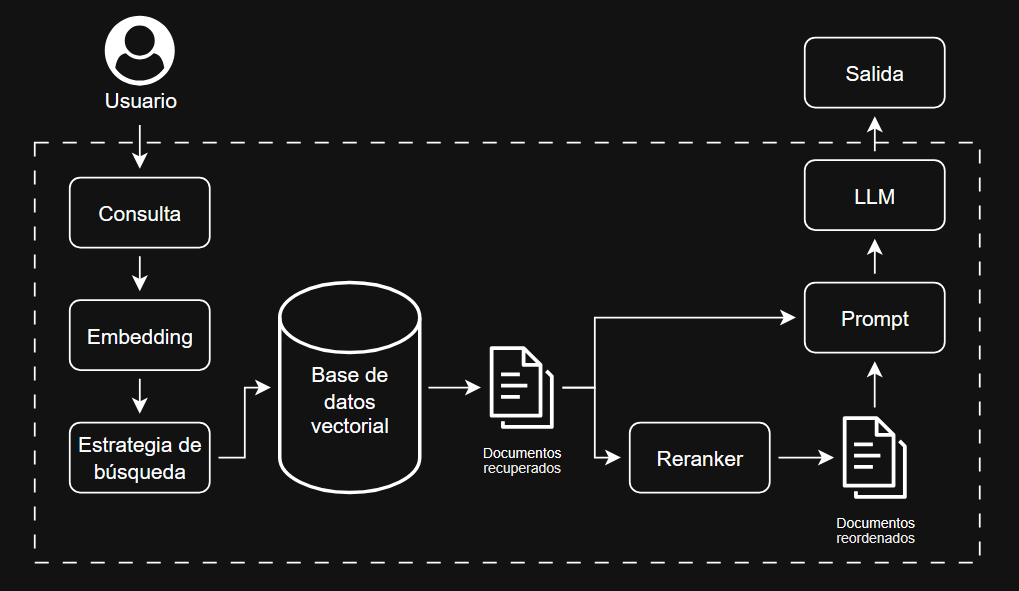
\includegraphics[width=0.8\textwidth]{imagenes/0052_estructura.png}
            \caption{Arquitectura de nuestro sistema RAG}		
            \label{fig:0052_estructura}
        \end{figure} 

        \noindent La consulta de usuario es vectorizada con el mismo modelo de embedding que hemos usado para la construcción de la base de datos vectorial para una mejor integridad de la respuesta, después es lanzada a la base de datos vectorial junto con la estrategia de búsqueda deseada.

        \noindent Los documentos recuperados son agregados al prompt para generar la respuesta usando el LLM que el usuario indique. Otra opción disponible en nuestro sistema, es la de usar un modelo de \textit{reranking} que filtre los documentos recuperados y seleccione los mejores para proporcionárselos de la misma manera al LLM mediante el prompt.

        \noindent La salida generada mostrará la información necesaria para responder a la entrada del usuario teniendo en cuenta el contenido relevante aportado por los documentos devueltos por el modelo de recuperación de información.

    \section{Planificación y presupuesto}
    
    	En esta sección explicaremos la planificación seguida en el proyecto, la metodología usada y todas las fases por las que pasamos durante el proceso de desarrollo de nuestra aplicación. Terminaremos la sección planteando el presupuesto estimado del proyecto, basándonos en los días transcurridos y en los integrantes pertenecientes al equipo de desarrollo.
    
    	\subsection{Metodología seguida: Scrum}

	        El proyecto se planifico desde un principio siguiendo el enfoque de las metodologías ágiles o \textbf{Scrum}. Este es un proceso en el que se aplican de manera regular un conjunto de buenas prácticas para trabajar colaborativamente, en equipo, y obtener el mejor resultado posible de un proyecto \cite{0028_scrum}. Aunque el ámbito de este Trabajo de Fin de Máster es individual, este proceso se sigue en la gran mayoría de empresas del sector de las tecnologías de la información, por lo que es interesante explorar su uso en el desarrollo de este proyecto.
	
	        \noindent Para llevar a cabo este seguimiento se propuso el uso de la herramienta \textit{Jira}, la cuál ofrece plantillas para crear la planificación de un proyecto siguiendo la metodología Scrum (figura \ref{fig:0053_jira-scrum}). Además, esta herramienta permite la conexión con repositorios de \textit{GitHub} (figura \ref{fig:0054_jira-github}) y asignar ramas de nuestro repositorio a las tareas contenidas en los tableros del sprint, de esta manera podemos mantener un cierto seguimiento en el avance del desarrollo en ambas plataformas.    
	
	        \begin{figure}[H]
	            \centering
	            
\includegraphics[width=0.7\textwidth]{imagenes/0053_jira-scrum.png}
	            \caption{Jira. Plantilla Scrum para el proyecto}		
	            \label{fig:0053_jira-scrum}
	        \end{figure} 
	
	        \begin{figure}[H]
	            \centering
	            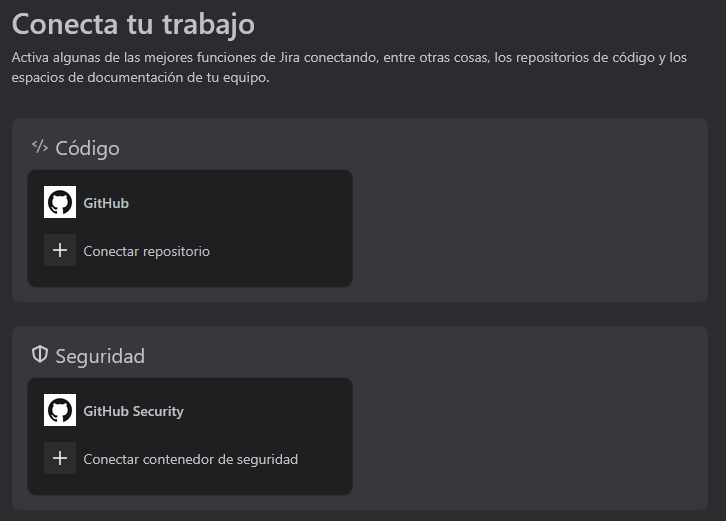
\includegraphics[width=0.6\textwidth]{imagenes/0054_jira-github.png}
	            \caption{Jira. Conexión con la plataforma de control de versiones GitHub}		
	            \label{fig:0054_jira-github}
	        \end{figure}         
	
	        \noindent En Scrum, un proyecto se ejecuta en ciclos temporales cortos y de duración fija llamados \textit{sprints}. En nuestro caso, estas iteraciones variaron entre 1, 2 o hasta 4 semanas dependiendo de la carga de trabajo o las tareas correspondientes al sprint. Cada sprint culminaba en una reunión presencial o vía telemática. donde se anunciaban los progresos alcanzados en el sprint, y se planeaban los objetivos para el siguiente.     
	
	        \noindent La figura \ref{fig:0056_jira-backlog} muestra la pestaña de \textit{Backlog}. Esta pestaña muestra en la parte superior todas las tareas que se tienen que cumplir en el sprint actual; y en la inferior, las tareas pendientes para futuros sprints. 
	
	        \begin{figure}[H]
	            \centering
	            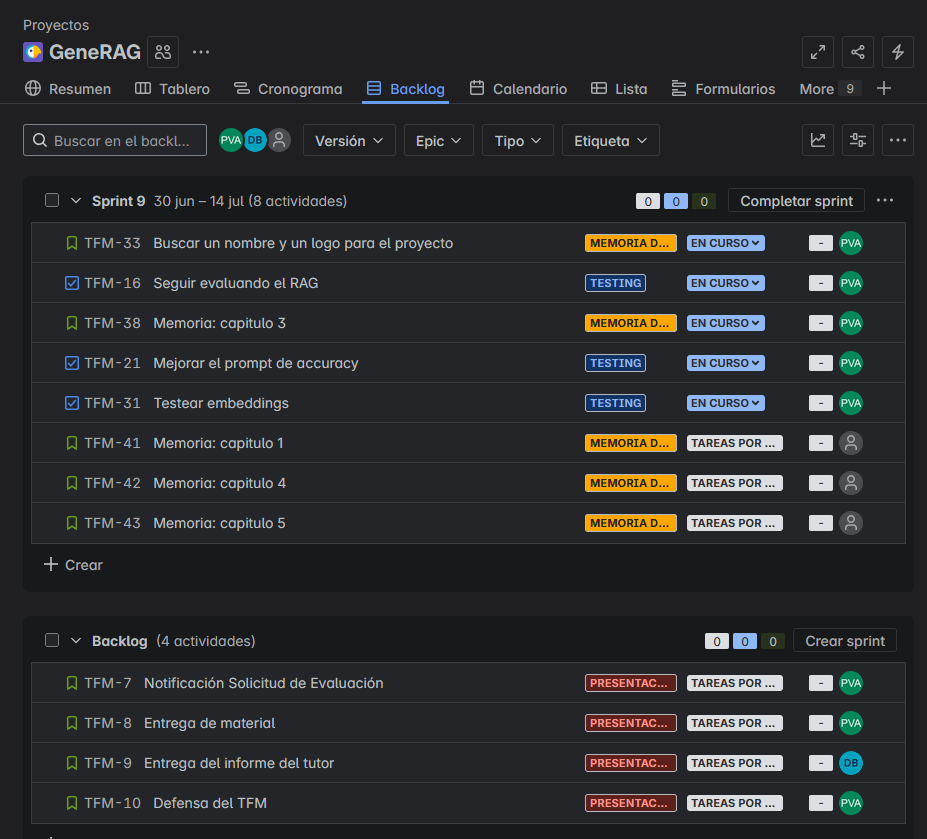
\includegraphics[width=0.7\textwidth]{imagenes/0056_jira-backlog.png}
	            \caption{Jira. Pestaña Backlog, tareas del sprint 9 y pendientes \cite{0056_proyectoJIRA}}		
	            \label{fig:0056_jira-backlog}
	        \end{figure} 
	
	        \noindent Una vez iniciado el sprint, en la pestaña \textit{Tablero} (figura \ref{fig:0058_jira-sprint2}) podemos ver las tareas asignadas anteriormente en el backlog y las columnas ``POR HACER", ``EN CURSO", ``EN REVISIÓN", y ``LISTO", columnas que podemos editar y añadir más. La lógica de estas columnas es mantener un control sobre que tarea se esta haciendo en este momento y quien es el encargado de ella. Cada tarea va avanzando hacia la columna de su derecha donde será evaluada hasta llegar a "LISTO", cuando podremos considerar la tarea acabada.        
	
	        \begin{figure}[H]
	            \centering
	            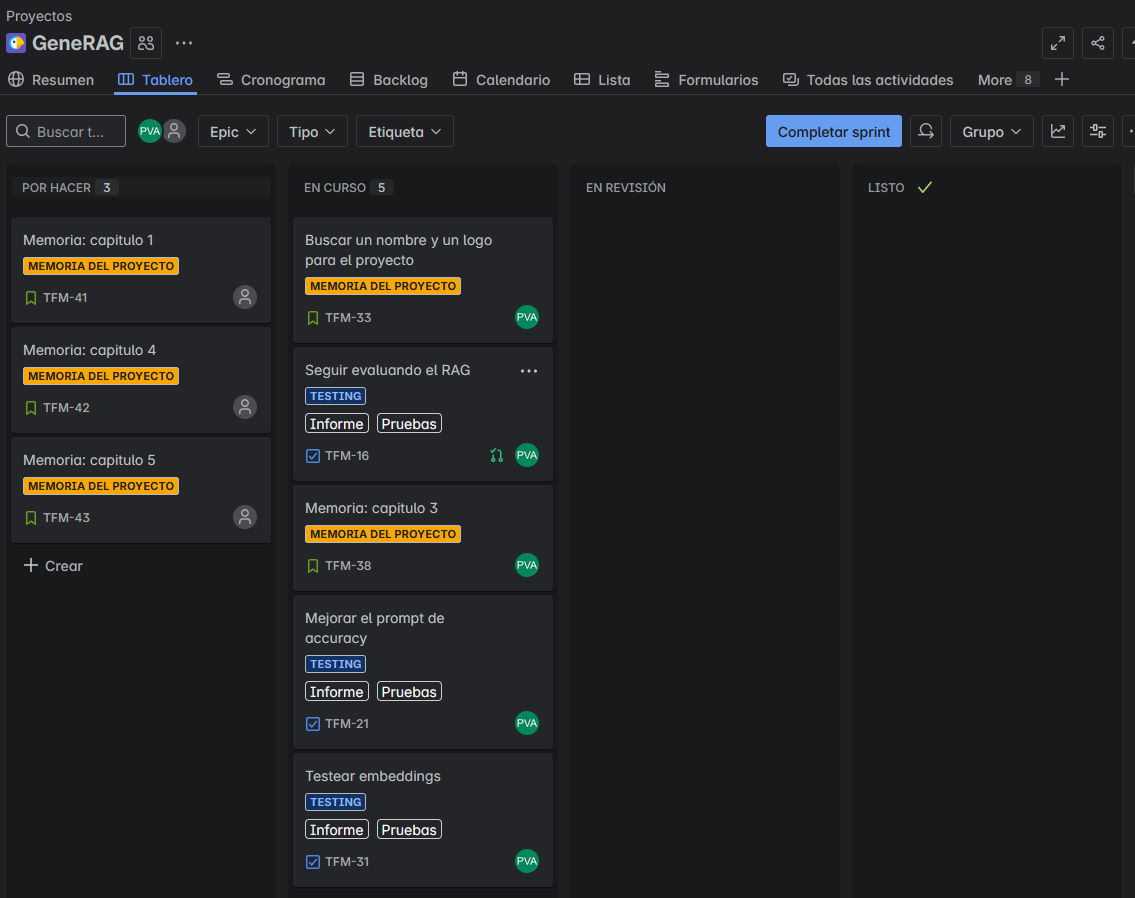
\includegraphics[width=0.8\textwidth]{imagenes/0058_jira-sprint2.png}
	            \caption{Jira. Tablero con tareas}		
	            \label{fig:0058_jira-sprint2}
	        \end{figure}         
	        
	        \noindent Por último, podemos ver el progreso en el tiempo de nuestro proyecto en la pestaña \textit{Cronograma} \cite{0056_proyectoJIRA}, el cual será explicado en la siguiente sección.
	        
      	\subsection{Fases del proyecto}      	  
      	
      		Las siguientes subsecciones explican brevemente lo realizado durante las distintas fases del proyecto, desde el inicio de la idea para el proyecto hasta su conclusión y entrega \cite{0056_proyectoJIRA}. En la figura \ref{fig:0139_crono}, observamos las fases por las que pasó el proyecto, su duración y los sprints totales. La duración total del proyecto ha sido de 204 días.     
      		
      		\begin{figure}[H]
      			\centering
      			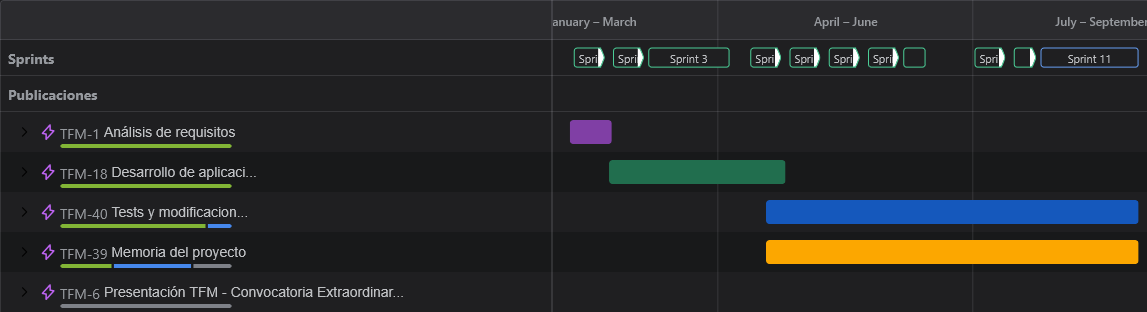
\includegraphics[width=1\textwidth]{imagenes/0139_crono.png}
      			\caption{Cronograma del proyecto. Extraído del proyecto en Jira \cite{0056_proyectoJIRA}}		
      			\label{fig:0139_crono}
      		\end{figure}          
        
        	\subsubsection{Fase 1: Análisis de requisitos} 
        	
        		En esta fase se presenta la idea del proyecto. Al principio, la idea era seguir experimentando con la plataforma RASA e iniciar un nuevo proyecto dedicado a crear un chatbot dedicado a un dominio en específico. 
        		
        		\noindent Pronto, la idea giró en torno a la utilización de los LLMs, dado a que era y es una tecnología en auge que presenta una mejora notable tanto en eficiencia como en rendimiento a lo que ofrece RASA en estos momentos. En este tiempo se realizaron varias demos usando las plataformas RASA y LangChain, decidiéndose por usar esta última en el proyecto.
        		
        		\noindent En la reunión que marcaba el final de sprint y de la fase, se determinó el propósito del chatbot: crear un asistente virtual capaz de responder con precisión y eficacia a cualquier pregunta relacionada con la DANA. Para ello, debíamos crear un RAG con los documentos del BOE relacionados con este tema. Además, nuestro tutor nos propuso la tarea de medir el grado de acierto del sistema RAG mediante el uso de agentes críticos. 
        		
        		\noindent Así pues, el proyecto quedó definido: crear un RAG sobre el contexto específico de la DANA, y medir su rendimiento evaluándolo a través de agentes críticos.
        		
        	\subsubsection{Fase 2: Desarrollo de la aplicación}
        	
        		En esta fase intermedia del proyecto, avanzamos en el desarrollo de la aplicación. Los cambios y adicciones al proyecto eran mostrados en las reuniones de finales de sprint, en las cuales se planteaban nuevas soluciones a las dificultades encontradas y se fijaban nuevos objetivos para el siguiente sprint. En esta etapa se completo el sistema RAG desde cero, desarrollo que se describe a continuación.
        		
        		\noindent El primer escollo, fue conseguir la fuente de conocimiento. Gracias a que los documentos del BOE se pueden conseguir vía API, se facilitó este primer problema. Fueron diseñados varios scripts para conseguir de forma automática estos documentos, y con la ayuda de \textit{GitHub Actions}, fueron programados para ejecutarse una vez al día salvo los domingos. De esta forma, obtuvimos la fuente de conocimiento que necesitaba nuestro RAG.
        		
        		\noindent La creación del RAG no tuvo mucha complicación debido a la gran cantidad de tutoriales y la versatilidad que nos permite LangChain en este contexto. La primera versión sin interfaz, era totalmente funcional en apenas unos días.
        		
        		\noindent En la interfaz empleamos más tiempo, dado a que la librería usada (Streamlit) ofrece bastantes elementos de personalización. La versión final permite cambiar el modelo de lenguaje usado para generar la respuesta, y también, elegir la estrategia de búsqueda empleada por el modelo de recuperación. En la parte de creación y actualización de la base de conocimientos, usamos dos alternativas para subir documentos desde la propia interfaz: desde carpeta o desde ficheros individuales.
        		
        		\noindent Completada esta fase, ya teníamos un sistema RAG totalmente funcional, con su fuente de conocimiento y una interfaz para responder consultas o añadir más documentos.
        		
        	\subsubsection{Fase 3: Test y modificaciones}
        	
        		Esta es la etapa de más duración del proyecto, y en la cual se realizaron todos los test para completar el segundo objetivo del trabajo.
        		
        		\noindent En primera instancia, desarrollamos un pequeño script diseñado para generar un conjunto de preguntas extraídas de nuestra fuente de conocimiento. Para su obtención, usamos el modelo de lenguaje Mistral Small 3.2, en el cual configuramos un prompt para este cometido. El conjunto de preguntas conseguido fue el usado para elaborar los test.
        		
        		\noindent Seguidamente, se preparó otro script en el que se configuró todo lo necesario para evaluar el RAG. Se definieron cuatro agentes críticos destinados a evaluar las métricas de \textit{accuracy}, \textit{faithfulnes}, \textit{groundedness} y \textit{relevancia}, es decir, el grado de similitud de la respuesta generada con la esperada, el uso de las evidencias proporcionadas por el modelo de recuperación en la respuesta generadas, y como de relevantes son los documentos recuperados para responder a la consulta.
        		
        		\noindent Las pruebas tomaron bastante tiempo debido al número realizado. Cada prueba de Mistral Small 3.2 empleaba alrededor de 3 horas en realizarse cuando el modelo estaba disponible, en ocasiones el servicio era más lento o fallaba. Llama 3.2 gastaba más o menos el mismo tiempo y GPT-4.1 era el más rápido (40 minutos), aunque para estos usamos conjuntos de pruebas más pequeños. Los resultados obtenidos fueron guardados y expuestos en tablas y gráficas, observables en el siguiente capítulo de esta memoria. 
        	
        	\subsubsection{Fase 4: Documentación}
        	
        		Esta fase se realizó en conjunto con la anterior (fase 3), por eso tiene más o menos la misma duración que esta. 
        		
        		\noindent En la estructura seguimos como guía la memoria usada en mi TFG, añadiendo y quitando las secciones que creímos necesarias.

        \subsection{Presupuesto}
        
        	En este apartado se describen los distintos recursos hardware y software empleados en el desarrollo del proyecto, explicando su uso y el coste de estos.
        	
        	\subsubsection{Recursos hardware}
        	
        		La tabla \ref{tab:rec_hard} muestra los recursos hardware usados. Para calcular el coste total de la tabla \ref{tab:presu_hard}, hemos dividido el precio entre la vida útil de cada dispositivo en días, para después multiplicarlo por el tiempo de realización del proyecto (204 días).
        		
        		\begin{table}[H]
        			\centering
        			\tiny
        			\begin{tblr}{
        					colspec = {p{2.5cm} p{3.5cm} p{7cm}},
        					row{1} = {bg=green!50}, 
        					hlines,
        					vlines,
        				}
        				\textbf{Dispositivo} & \textbf{Modelo} & \textbf{Uso} \\
        				Ordenador sobremesa & Ryzen5 3600 + 32GB RAM + 6700XT 12GB VRAM & Desarrollo y prueba de la aplicación \\
        				Ordenador portátil & Ryzen7 6800HS + 16GB RAM & Desarrollo y prueba de la aplicación \\        				
        			\end{tblr}
        			\caption{Recursos hardware utilizados}
        			\label{tab:rec_hard}
        		\end{table}
        		
        		\begin{table}[H]
        			\centering
        			\tiny
        			\begin{tblr}{
        					colspec = {p{6.5cm} p{2cm} p{2cm} p{2cm}},
        					row{1} = {bg=green!50}, 
        					row{4} = {bg=green!10}, 
        					hlines,
        					vlines,
        				}
        				\textbf{Modelo} & \textbf{Precio} & \textbf{Vida útil} & \textbf{Total} \\
        				Ryzen5 3600 + 32GB RAM + 6700XT 12GB VRAM & 1500€ & 8 años & 104.8€ \\
        				Ryzen7 6800HS + 16GB RAM & 1000€ & 6 años & 94.15€ \\     
        				\SetCell[c=3]{wd=10.5cm,valign=t}\textbf{Total} & & & \textbf{198.95€} \\		
        			\end{tblr}
        			\caption{Presupuesto de los recursos hardware utilizados}
        			\label{tab:presu_hard}
        		\end{table}
        		
        	\subsubsection{Recursos software}
        		
        		En este apartado se describen los recursos software utilizados, tanto su uso en la tabla \ref{tab:rec_soft}, como su precio en la tabla \ref{tab:presu_soft}. Los precios de estos recursos van ligados al coste de su licencia o uso.
        		
        		\begin{table}[H]
        			\centering
        			\tiny
        			\begin{tblr}{
        					colspec = {p{3cm} p{10cm}},
        					row{1} = {bg=green!50}, 
        					hlines,
        					vlines,
        				}
        				\textbf{Herramienta} & \textbf{Uso} \\
        				Windows 11 & Sistema Operativo \\    				
        				Visual Studio Code & Entorno de desarrollo \\
        				Ollama & Gestor de LLM y embeddings \\
        				LangChain & Librería control LLM \\
        				Streamlit & Librería interfaz \\
        				GitHub \& GitHub Actions & Plataforma donde esta el repositorio del proyecto, y plataforma para crear automatizaciones \\
        				Mistral API & Uso de LLMs de Mistral \\
        				OpenAI API & Uso de LLMs y embeddings de OpenAI \\
        				TexStudio & Procesador de látex usado para elaborar la memoria \\
        			\end{tblr}
        			\caption{Recursos software utilizados}
        			\label{tab:rec_soft}
        		\end{table}
        		
        		\begin{table}[H]
        			\centering
        			\tiny
        			\begin{tblr}{
        					colspec = {p{3cm} p{10cm}},
        					row{1} = {bg=green!50}, 
        					row{11} = {bg=green!10},
        					hlines,
        					vlines,
        				}
        				\textbf{Herramienta} & \textbf{Uso} \\
        				Windows 11 & 145€ \\    				
        				Visual Studio Code & Gratuito \\
        				Ollama & Gratuito \\
        				LangChain & Gratuito \\
        				Streamlit & Gratuito \\
        				GitHub \& GitHub Actions & Gratuito\\        				
        				Mistral API & Gratuito \\
        				OpenAI API & 12,79€ (15\$) \\
        				TexStudio & Gratuito \\
        				\textbf{Total} & \textbf{157.79€}
        			\end{tblr}
        			\caption{Presupuesto de los recursos software utilizados}
        			\label{tab:presu_soft}
        		\end{table}
        		
        	\subsubsection{Recursos personales}
        	
        		En este apartado describiremos los miembros presentes en la realización del proyecto. En la tabla \ref{tab:rec_ presu_pers} tendremos en cuenta el puesto, tiempo invertido y coste de ese tiempo. 
        		
        		\noindent Las horas realizadas por los tutores se han calculado teniendo en cuenta una media de una hora por reunión. De un total de 15 sesiones de reunión, disponemos de un total de 900 minutos o 15 horas. 
        		
        		\noindent El coste de su salario, se ha estimado sabiendo el salario bruto aproximado de un profesor de universidad (31500€ anuales, 24500€ netos según el IRPF de 2024). Por lo que, en un horario normal de 40 horas semanales, habiendo 4.34 semanas/mes , asciende a 11.76€ por hora. 
        		
        		\noindent Para el cómputo de mis horas, conociendo la duración del proyecto y en una media de 3 horas de trabajo al día, tenemos un total de 612 horas aproximadamente. El salario medio de un  programador junior ronda los 1500€, así que podemos estimar  un salario medio por hora de 8.64€, y un total de 5.287,68€.
        	
        		\begin{table}[H]
        			\centering
        			\tiny
        			\begin{tblr}{
        					colspec = {p{3cm} p{5.5cm} p{1cm} p{1cm} p{1cm}},
        					row{1} = {bg=green!50}, 
        					row{5} = {bg=green!10},
        					hlines,
        					vlines,
        				}
        				\textbf{Nombre} & \textbf{Puesto} & \textbf{Tiempo} & \textbf{Coste} & \textbf{Total}\\
        				David Griol Barres & Profesor de Universidad & 15h & 11.76€/h & 176.4€ \\
        				Zoraida Callejas Carrión & Profesor de Universidad& 15h & 11.76€/h & 176.4€ \\
        				Pablo Valenzuela Álvarez & Programador Junior & 612h & 8.64€ & 5.287,68€ \\
        				\SetCell[c=4]{wd=10.5cm,valign=t}\textbf{Total} & & & & \textbf{5.640,48€}\\
        			\end{tblr}
        			\caption{Presupuesto de los recursos personales utilizados}
        			\label{tab:rec_ presu_pers}
        		\end{table}
        	
        	\subsubsection{Coste total}
        	
        		Sumando todos los costes parciales del proyecto, tenemos un subtotal de 5.997,22€.
        		
        		\begin{table}[H]
        			\centering
        			\tiny
        			\begin{tblr}{
        					colspec = {p{6cm} p{7cm}},
        					row{1} = {bg=green!50}, 
        					row{5} = {bg=green!10},
        					hlines,
        					vlines,
        				}
        				\textbf{Tipo} & \textbf{Coste} \\
        				Coste del hardware & 198.95€ \\    				
        				Coste del software & 157.79€ \\    				
        				Coste del personal & 5.640,48€ \\    				
        				\textbf{Total} & \textbf{5.997,22€}
        			\end{tblr}
        			\caption{Coste total del proyecto}
        			\label{tab:presu_total}
        		\end{table}
        		
    \section{Construcción del corpus de documentos}

        La plataforma elegida para el control de versiones del proyecto fue \textit{GitHub}, ya que es la plataforma con la que llevamos años trabajando en proyectos anteriores y es la más implantada en el mercado. 
        
        \noindent A parte de dar un acceso rápido y seguro al código del repositorio, \textit{GitHub} ofrece una herramienta para controlar flujos de trabajo automáticos llamada \textbf{GitHub Actions}. Flujos que hemos usado para automatizar las descargas de los documentos usados para crear el corpus de información con la que hemos nutrido el modelo de recuperación de información de nuestro sistema RAG. Este es un concepto conocido como integración continua y entrega continua (\textit{CI/CD}).

        \noindent Como se ha mencionado en anteriores apartados, hemos usado documentos del BOE (Boletín Oficial del Estado) relacionados con la DANA para construir nuestro corpus de conocimiento. Desde la propia web del BOE, podemos acceder a los sumarios de cada día mediante descarga gracias a una API.       

        \begin{figure}[H]
            \centering
            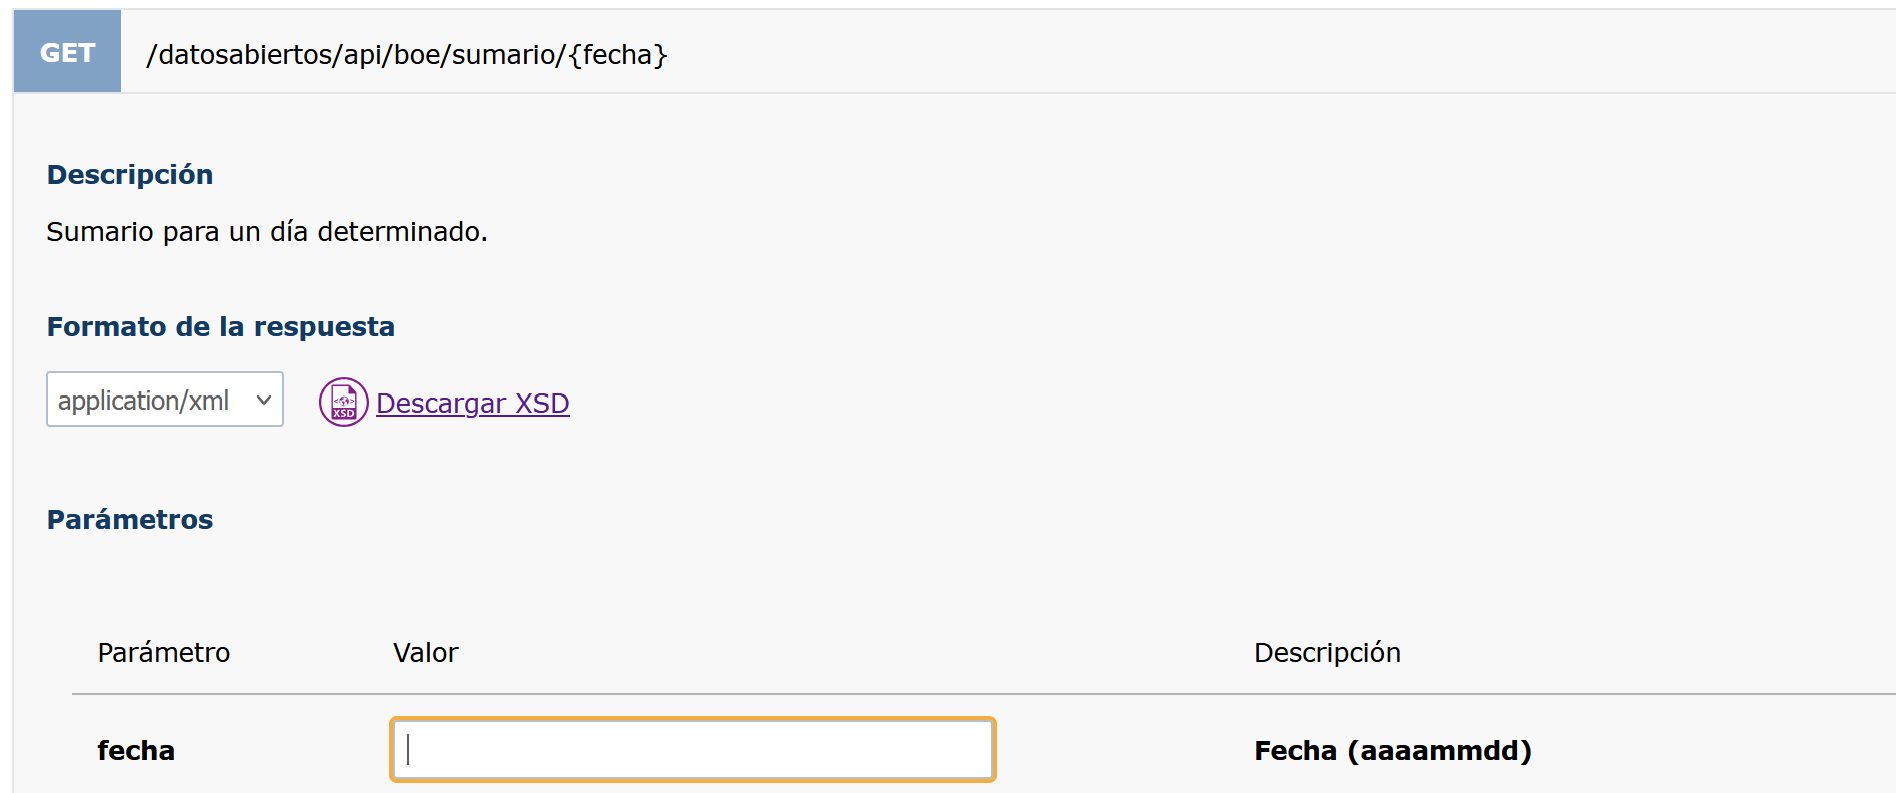
\includegraphics[width=1\textwidth]{imagenes/0059_boe_api.png}
            \caption{BOE. API web desde la que descargar sumarios por día \cite{0029_boe_api}}		
            \label{fig:0059_boe_api}
        \end{figure} 

        \begin{figure}[H]
            \centering
            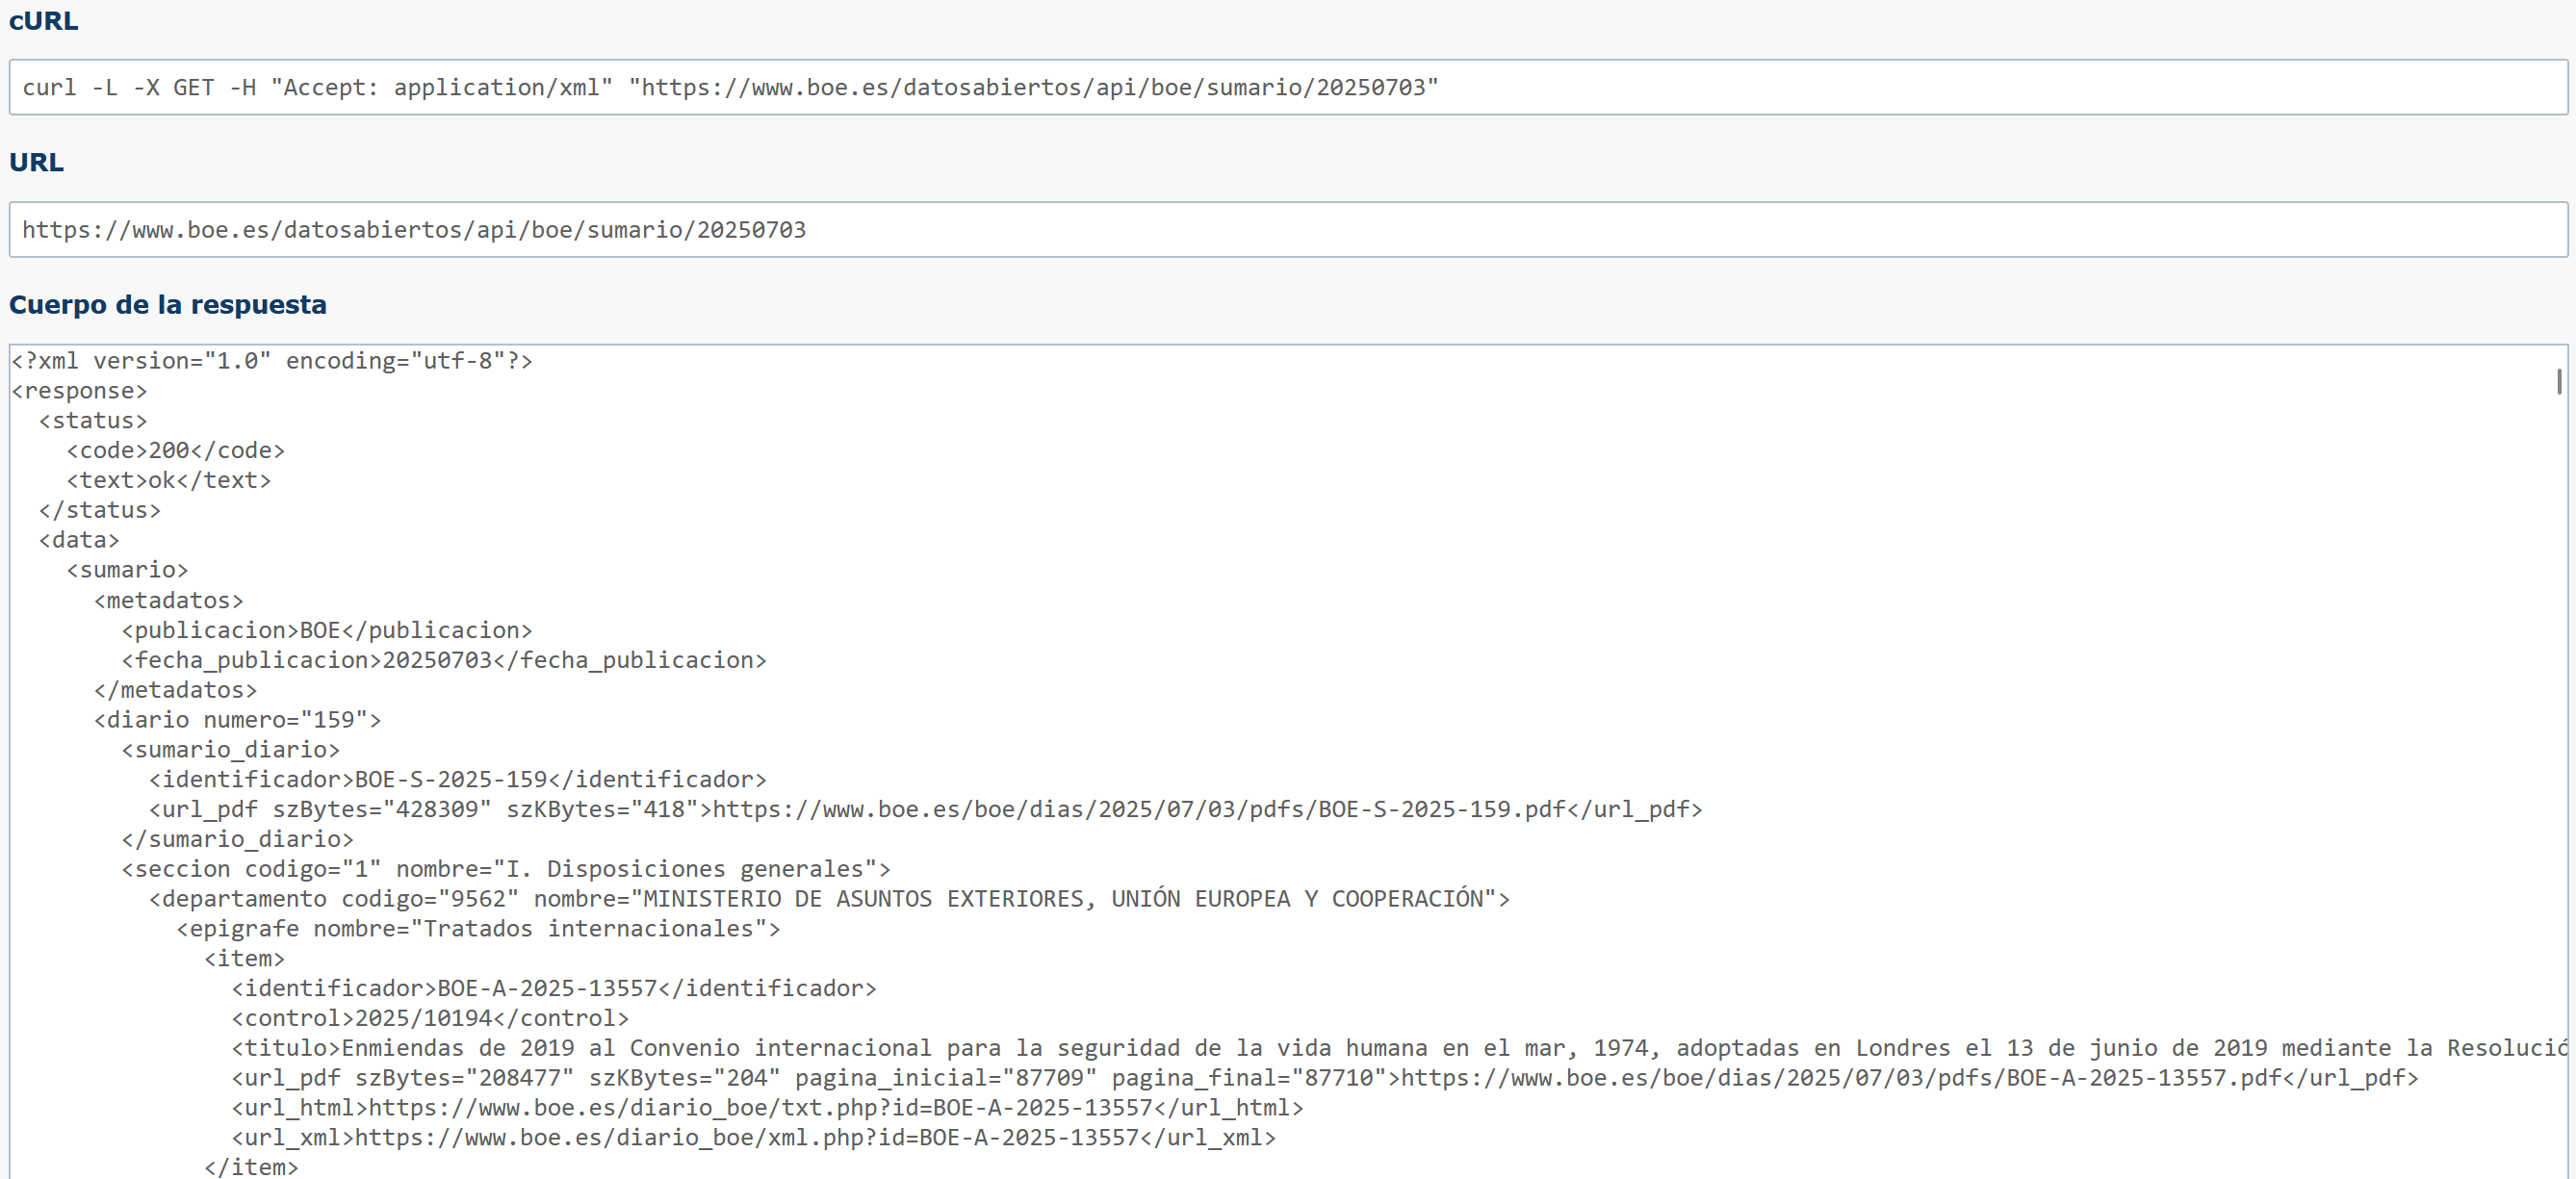
\includegraphics[width=1\textwidth]{imagenes/0060_boe_api2.png}
            \caption{BOE. Resultados de la búsqueda de un día \cite{0029_boe_api}}		
            \label{fig:0060_boe_api2}
        \end{figure} 

        \noindent Esta API nos ofrece dos opciones de descarga para el sumario: json y xml. En la figura \ref{fig:0060_boe_api2} podemos ver la versión xml de la descarga.

        \noindent El requerimiento para la obtención del sumario es la fecha redactada en un formato \textbf{aaaammdd}, es decir, si queremos obtener el sumario del día 30 de mayo de 2025, tenemos que redactarlo de la siguiente manera: 20250530.

        \subsection{Script de descarga de sumarios}
        \label{subsec:3_script_suma}

            La fecha del sistema es fácil de obtener mediante código, por dicha razón se implementaron dos scripts: uno para la descarga automática del sumario del día actual y otro para la descarga de sumarios de días anteriores, necesarios para el paso siguiente (ver sección \ref{subsec:3_script_docs}).
    
            \begin{figure}[H]
                \centering
                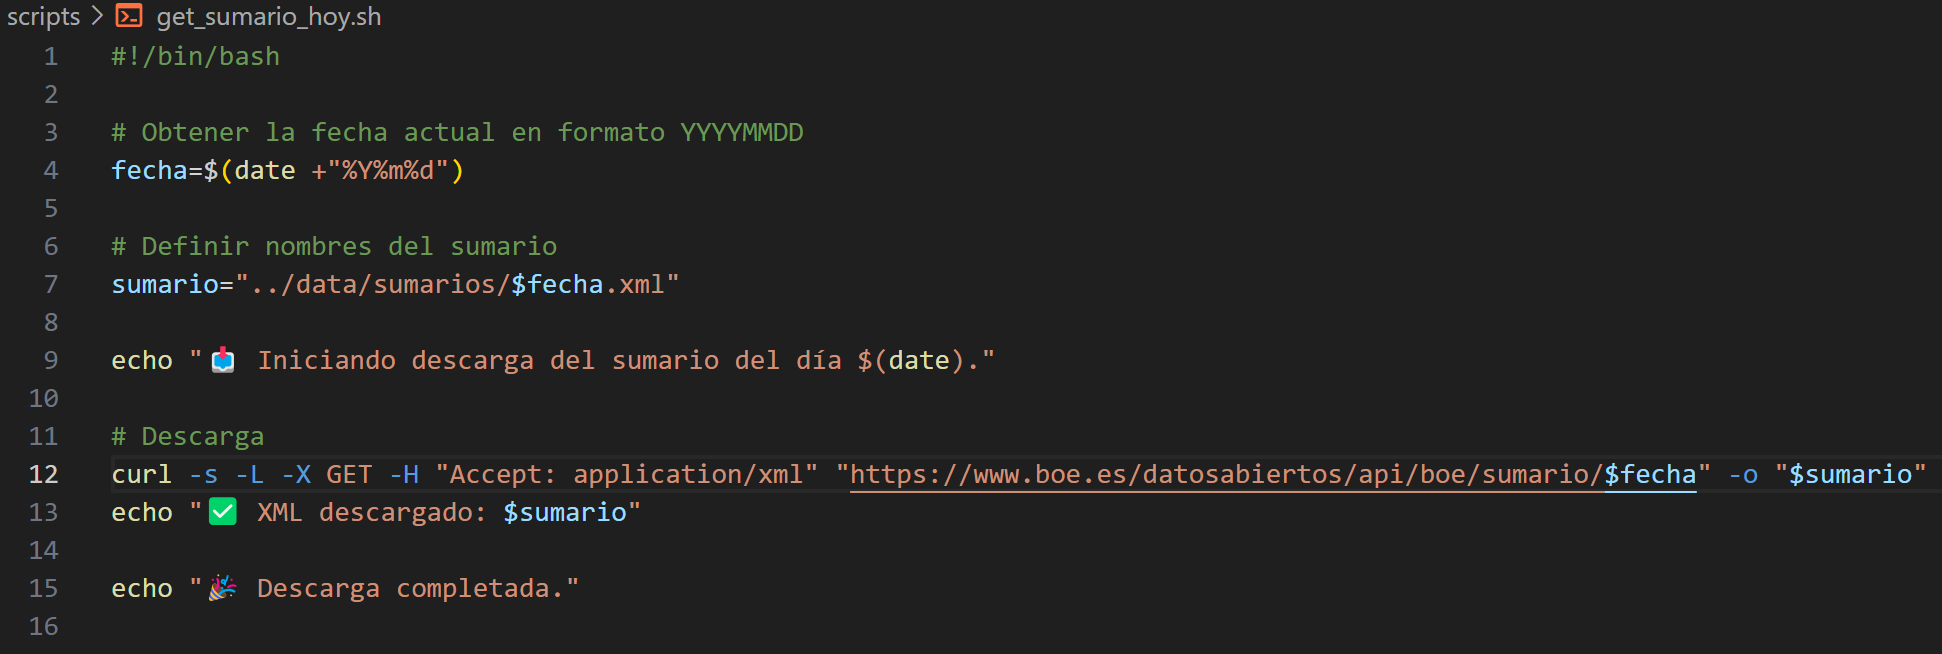
\includegraphics[width=0.9\textwidth]{imagenes/0061_get_sumario.png}
                \caption{Script para descargar el sumario del día}		
                \label{fig:0061_get_sumario}
            \end{figure} 
    
            \noindent Como se observa en la figura \ref{fig:0061_get_sumario}, se obtiene la fecha del sistema automáticamente y se usa tanto para la llamada a la API como para guardar el documento descargado. Este script es el se usó posteriormente para crear hacer una automatización por medio de GitHub Actions (ver sección \ref{subsec:3_subsec_auto}).

        \subsection{Script para la descarga de documentos}
        \label{subsec:3_script_docs}

            Los sumarios en su estructura xml contienen varias etiquetas que podemos usar para buscar y descargar los documentos que nos interesen. Como podemos observar en la figura \ref{fig:0060_boe_api2}, la etiqueta \textit{item} engloba tanto las etiquetas del título como varias etiquetas de descargas. Ayudándonos de estas etiquetas, se optó por crear un script en Python que automatizase el proceso de descarga de los documentos relacionados con la DANA.

            \noindent El funcionamiento de este script es el siguiente:

            \begin{itemize}
                \item Recorremos en bucle todas las etiquetas ``\textit{item}"
                \item Para cada etiqueta ``\textit{item}" se guardan en variables: título y enlace de descarga pdf.
                \item Se comprueba si el título contiene la palabra ``DANA".
                \item Se descarga el documento gracias a la etiqueta del enlace pdf.
            \end{itemize}     

            \noindent En la figura \ref{fig:0062_get_docs} se puede observar este procedimiento.
    
            \begin{figure}[H]
                \centering                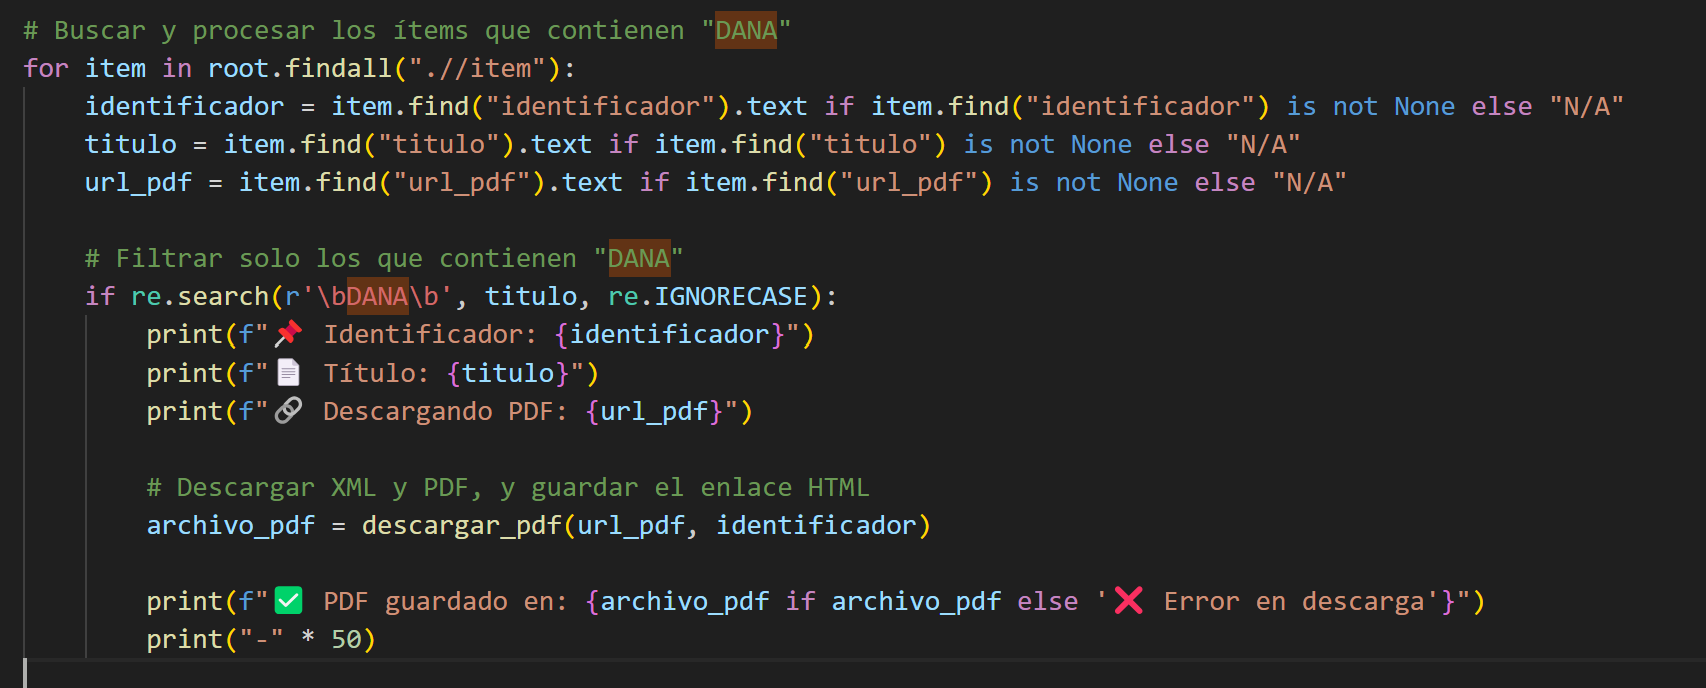
\includegraphics[width=0.8\textwidth]{imagenes/0062_get_docs.png}
                \caption{Fragmento del script encargado de obtener documentos relacionados con la DANA}		
                \label{fig:0062_get_docs}
            \end{figure} 

            \noindent Como sucedió en el apartado anterior, se hizo necesaria la implementación de otro script para la descarga de los documentos de días anteriores. El procedimiento es el mismo que el visto en la figura \ref{fig:0062_get_docs}, añadiendo un bucle extra en el cual recorre todos los sumarios descargados. 
            
            \noindent Tanto estos como los scripts del apartado anterior, están disponibles en la carpeta \textbf{scripts} del repositorio \cite{0045_repo} en \textit{GitHub}.

        \subsection{Automatización de procesos de descarga}
        \label{subsec:3_subsec_auto}

            Una vez implementados los scripts para la descarga de sumarios y de documentos, llega la hora de crear la automatización en GitHub. Para ello usaremos la herramienta para crear acciones: \textit{GitHub Actions}.

            \noindent \textit{GitHub Actions} es una plataforma de integración y despliegue continuos (\textit{CI/CD}) que permite la automatización de flujos de trabajo \cite{0030_gh_actions}.
    
            \begin{figure}[H]
                \centering
                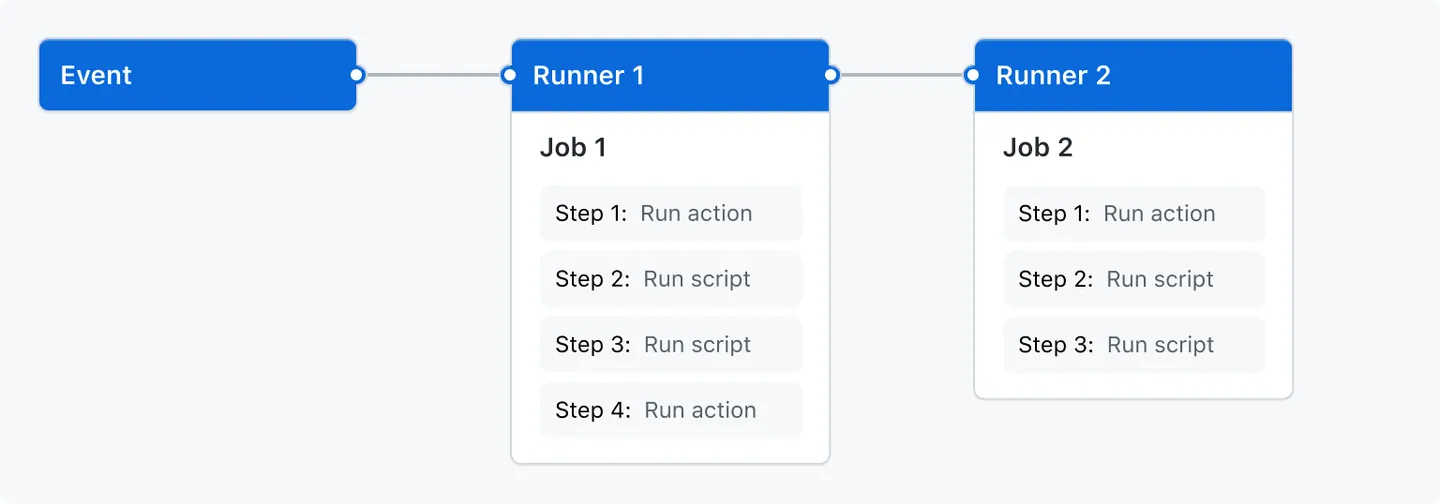
\includegraphics[width=0.8\textwidth]{imagenes/0063_ghact_fun.png}
                \caption{GitHub Actions. Ejemplo de funcionamiento de un flujo de trabajo \cite{0030_gh_actions}}		
                \label{fig:0063_ghact_fun}
            \end{figure} 

            \noindent Como se observa en la figura \ref{fig:0063_ghact_fun}, un flujo de trabajo (\textit{workflow}) se activa cuando sucede un evento (\textit{event}) en el repositorio: \textit{push}, \textit{commit}, etc. Cada trabajo (\textit{job}) ejecuta uno o varios scripts en una máquina virtual creada automáticamente que se elimina al completar los procesos del flujo de trabajo.

            \noindent Los flujos de trabajo son procesos automatizados y configurables definidos por un fichero \textit{YAML} ubicado en el directorio \textit{.github/workflow} de nuestro repositorio \cite{0045_repo}. Nuestro objetivo es que el flujo de trabajo se ejecute una vez al día, exceptuando los domingos (no se publica el BOE los domingos); y que ejecute ambos scripts vistos en las dos secciones anteriores.

            \noindent En este sentido, tenemos que configurar un evento que haga que se ejecute todos los días exceptuando el domingo. Esto se logra usando el comando \textit{cron} como se muestra en la figura \ref{fig:0064_ghact_cron}. En dicha figura, se programa para ejecutarse de lunes a sábado a las 9:00 de la mañana, sin importar día o mes.
    
            \begin{figure}[H]
                \centering
                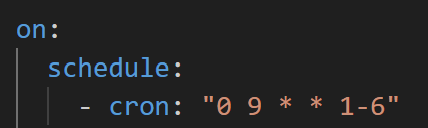
\includegraphics[width=0.4\textwidth]{imagenes/0064_ghact_cron.png}
                \caption{GitHub Actions. Fragmento del flujo de trabajo que muestra el uso del comando cron}		
                \label{fig:0064_ghact_cron}
            \end{figure}

            \noindent Tras programar el evento que activa el flujo de trabajo, solo queda indicar las tareas que se ejecutarán en el flujo. En la figura \ref{fig:0065_ghact_jobs} se pueden observar estas tareas bajo la etiqueta \textit{steps}, estos son iniciadas secuencialmente como indica la figura. En las primeras líneas, indica sobre que sistema se esta ejecutando: una máquina virtual Ubuntu.
    
            \begin{figure}[H]
                \centering
                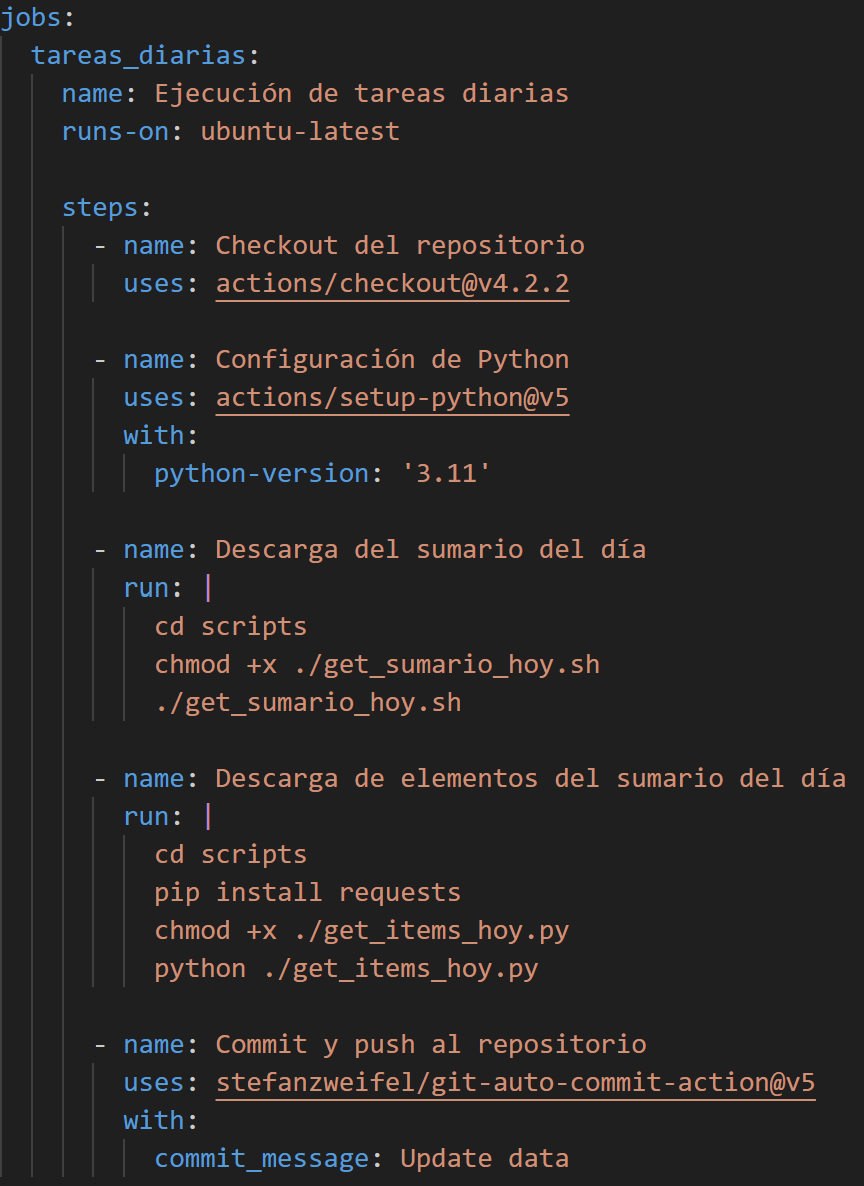
\includegraphics[width=0.5\textwidth]{imagenes/0065_ghact_jobs.png}
                \caption{GitHub Actions. Fragmento del flujo de trabajo que muestran los trabajos que son ejecutados}		
                \label{fig:0065_ghact_jobs}
            \end{figure}

            \noindent La lista siguiente contiene una breve descripción de cada una de las tareas del flujo por sus nombres:

            \begin{enumerate}
                \item \textbf{Checkout del repositorio}: Es una acción creada por la comunidad que clona el repositorio en la máquina virtual. 
                \item \textbf{Configuración de Python}: Utiliza otra acción creada por la comunidad, se encarga de instalar un entorno \textit{Python} en la máquina virtual.
                \item \textbf{Descarga del sumario del día}: Lanza el script de descarga del sumario del día (sección \ref{subsec:3_script_suma}).
                \item \textbf{Descarga de elementos del sumario del día}: Lanza el script de descarga de documentos del sumario del día relacionados con la DANA (sección \ref{subsec:3_script_docs}).
                \item \textbf{Commit y push al repositorio}: Ultiliza la acción \textit{auto-commit}, creada por la comunidad. Como su nombre indica, se encarga de actualizar los sumarios y documentos descargados, si hay nuevos.
            \end{enumerate}

            \noindent Para finalizar la subsección, queda comprobar si la acción se esta lanzando correctamente. Podemos obtener esta información en la pestaña ``Acciones" de la página web de \textit{GitHub} de nuestro repositorio \cite{0045_repo}. En las figuras siguientes podemos observar el funcionamiento de las acciones en el repositorio del proyecto \cite{0045_repo}.          
    
            \begin{figure}[H]
                \centering
                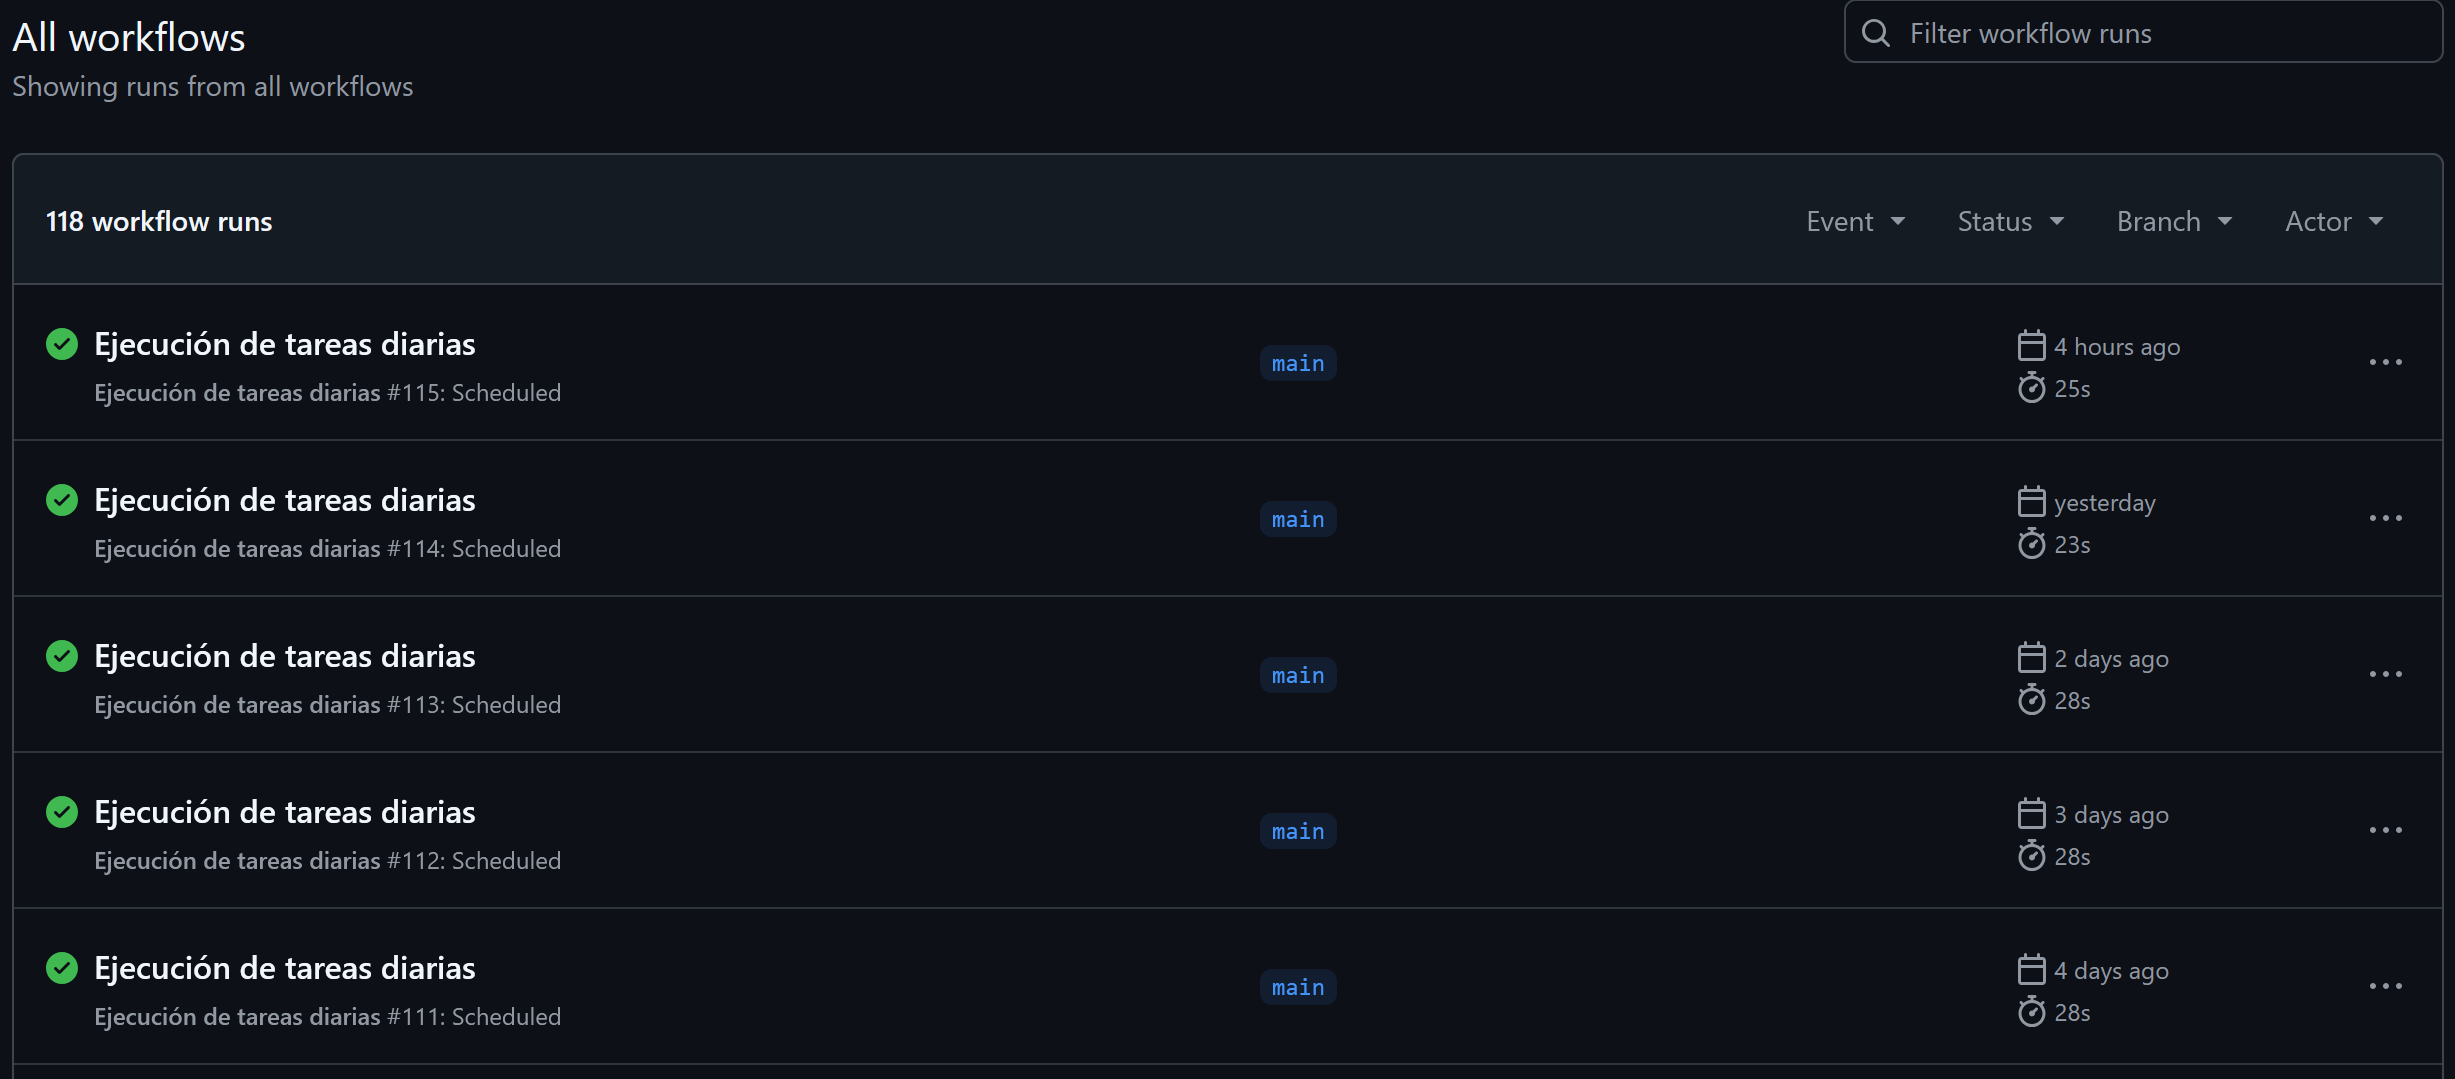
\includegraphics[width=0.8\textwidth]{imagenes/0066_ghact_allwf.png}
                \caption{Pestaña de acciones del proyecto. Se muestran una parte de las acciones automatizadas}		
                \label{fig:0066_ghact_allwf}
            \end{figure}        

            \noindent Podemos comprobar en la figura \ref{fig:0066_ghact_allwf} como, efectivamente, las acciones de lanzan una vez al día.
    
            \begin{figure}[H]
                \centering
                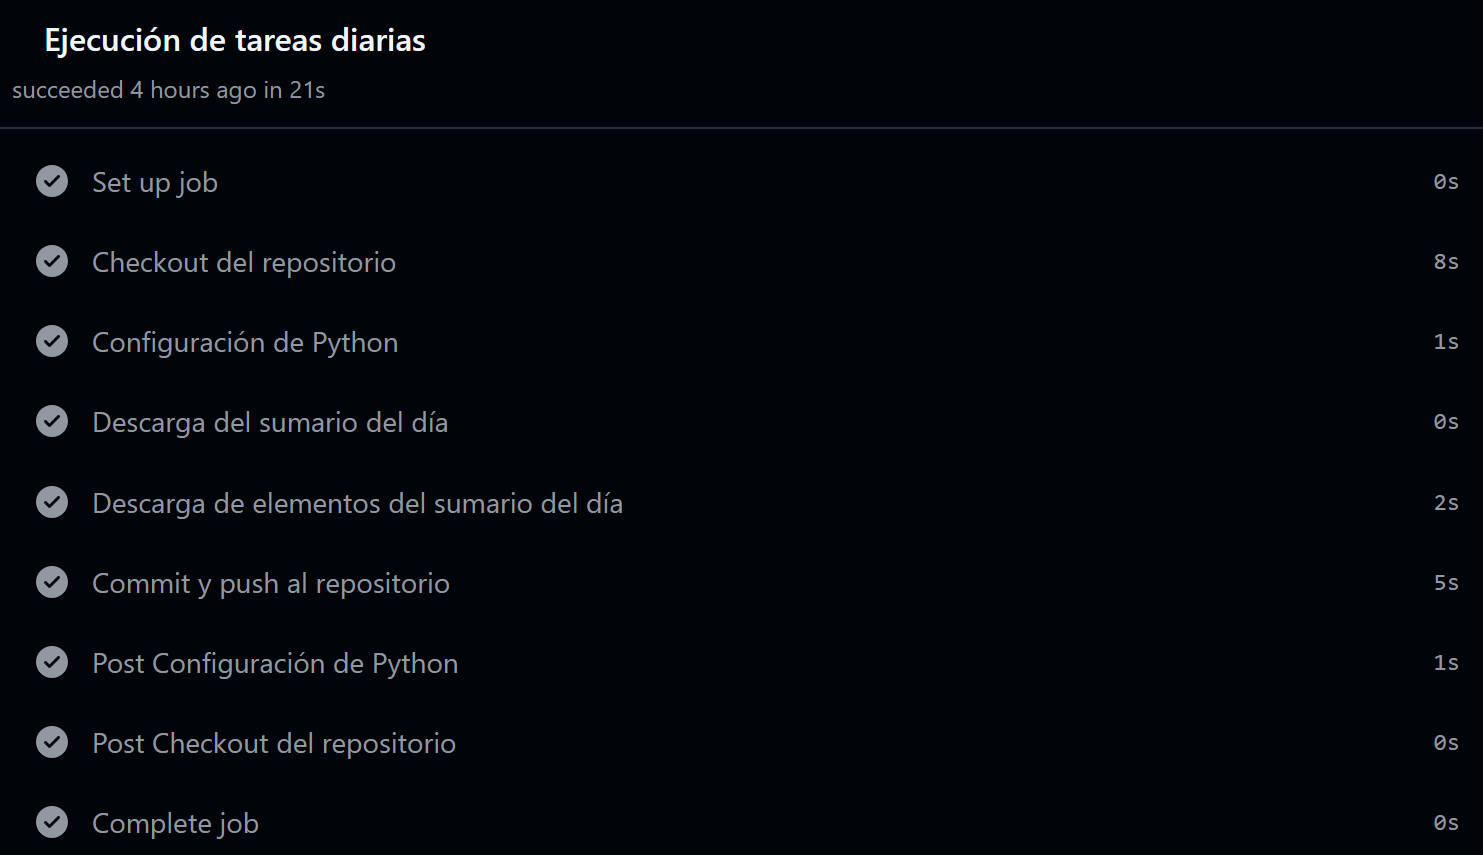
\includegraphics[width=0.8\textwidth]{imagenes/0067_ghact_finfin.png}
                \caption{Vista en detalle de una acción. Se observa el tiempo empleado en realizar cada paso}		
                \label{fig:0067_ghact_finfin}
            \end{figure}

            \noindent En la vista en detalle aportada en la figura \ref{fig:0067_ghact_finfin}, podemos entender como funciona internamente una acción, siguiendo los pasos indicados en el fichero \textit{YAML}. Los procesos \textit{post} se encargan de deshacer los procesos de \textit{checkout} y configuración de \textit{Python}, para terminar liberando la máquina virtual en el último paso. 

            \noindent De esta manera, hemos logrado crear una base de conocimiento con documentos del BOE relacionados con la DANA, y que es actualizada diariamente.

    \section{Desarrollo del chatbot}

        Esta sección contará los pasos que hemos seguido en el desarrollo de la aplicación chatbot que tiene de base nuestro sistema RAG. Encontraremos apartados dedicados tanto al desarrollo de la interfaz web como al de los diferentes componentes que configuran nuestro sistema RAG, incluyendo imágenes con fragmentos de código y de la interfaz final.

        \noindent El objetivo es crear una interfaz en la cuál: podamos añadir nuevos documentos a nuestro sistema RAG y, evidentemente, un chatbot con el que podamos comunicarnos, y que utilice documentos recuperados del RAG para construir su respuesta. Para dicho cometido se implemento una clase \textit{chatbot} (ubicada dentro de la carpeta \textit{classes} del repositorio \cite{0045_repo}), que contiene los métodos necesarios para hacer un funcionar el sistema RAG completo. 

        \noindent En las siguientes subsecciones mostraremos la implementación de estos procesos: la configuración, carga y agregación de nuevos documentos a la base de datos vectorial, y la recuperación y generación de información; todo ejemplificándolo con fragmentos de código representativos y muestras del resultado en la interfaz web.

        \subsection{Clase Chatbot: constructor}

            El constructor de la clase \textit{Chatbot}, como se observa en la figura \ref{fig:0068_chatbot_const_1}, contiene una gran cantidad de parámetros. Con ello podemos configurar desde la inicialización todos los aspectos necesarios del sistema RAG propuesto.

            \begin{figure}[H]
                \centering
                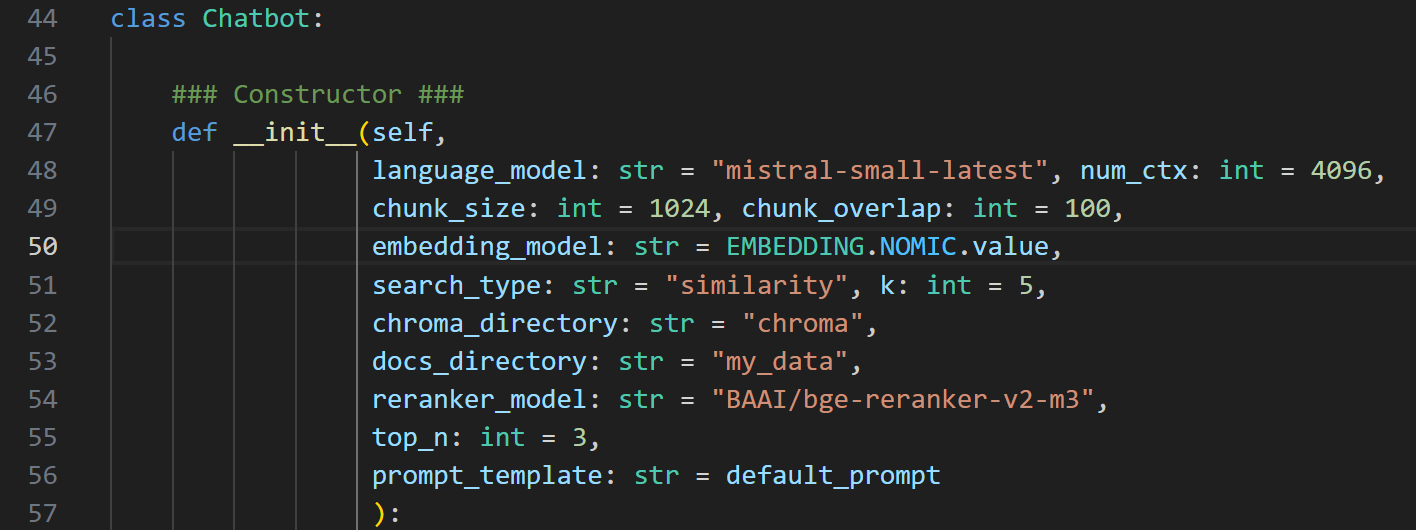
\includegraphics[width=1\textwidth]{imagenes/0068_chatbot_const_1.png}
                \caption{Clase Chatbot. Parámetros del constructor}		
                \label{fig:0068_chatbot_const_1}
            \end{figure}

            \noindent En la siguiente lista, vamos a explicar cada uno de los parámetros:

            \begin{itemize}
                \item \textbf{language\_model:} Indica el modelo de lenguaje (LLM) que usaremos para generar la respuesta.
                \item \textbf{num\_ctx:} Ventana de contexto que usa el LLM, es decir, la cantidad de información aportada al LLM mediante el prompt.
                \item \textbf{chunk\_size y chunk\_overlap:} Parámetros usados para separar y solapar documentos a la hora de añadirlos al RAG.
                \item \textbf{embedding\_model:} Modelo de embedding usado por el RAG, también es usado en las consultas de usuario.
                \item \textbf{search\_type y k:} Estrategia de búsqueda usada al recuperar información. La cantidad de documentos recuperados la indica k.
                \item \textbf{chroma\_directory:} Localización del modelo de recuperación (base de datos vectorial).
                \item \textbf{docs\_directory:} Localización del corpus usado, que nutre la base de datos vectorial.
                \item \textbf{reranker\_model y top\_n:} Modelo utilizado para hacer reranking sobre los documentos recuperados. La cantidad de documentos filtrados por el reranker la indica top\_n.
                \item \textbf{prompt\_template:} Plantilla de texto utilizada para generar la respuesta.
            \end{itemize}

            \noindent Como se observa en la imagen anterior cada parámetro usa valores por defecto, de esta manera se facilita el uso de esta clase. Cada uno de estos parámetros son editables en todo momento, puesto que se han incluido métodos \textit{GET} y \textit{SET} para estos cometidos.

            \noindent A continuación veremos en las figuras retazos de la configuración de alguno de ellos. Como por ejemplo la figura \ref{fig:0069_chatbot_const_2}, donde se muestra la configuración del modelo de lenguaje según sea el seleccionado. Hasta ahora contamos con el modelo \textit{mistral-small} correspondiente a MistralAI, \textit{GPT-4.1} de OpenAI y Llama3.2 perteneciente a Ollama, por lo que necesitamos diferentes clases para que funcionen: ChatMistralAI, ChatOpenAI y ChatOllama. En los modelos proporcionados por Mistral AI y OpenAI necesitamos facilitar la clave de su API.

            \begin{figure}[H]
                \centering
                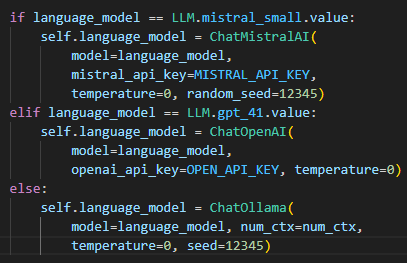
\includegraphics[width=0.6\textwidth]{imagenes/0069_chatbot_const_2.png}
                \caption{Clase Chatbot. Configuración del LLM}		
                \label{fig:0069_chatbot_const_2}
            \end{figure}

            \noindent En cuanto a la configuración del modelo de recuperación, la figura \ref{fig:0070_chatbot_const_3} muestra su implementación. La separación de documentos es efectuada mediante el uso de la clase \textit{RecursiveTextSplitting} \cite{0031_langchain_recursiveCS}, que se encarga de separar los documentos dado un determinado tamaño del chunk (\textit{chunk\_size}). El solapamiento se controla con \textit{chunk\_overlap}, este ayuda a mantener una relación semántica entre documentos similares o consecutivos.

            \noindent La figura \ref{fig:0070_chatbot_const_3} también muestra como se configura el modelo de embedding y la base de datos vectorial (\textit{vector\_store}); utilizando sendas clases \textit{OllamaEmbeddings} y \textit{Chroma} para realizar estas acciones. En el caso de usar un modelo de embedding proviniente de OpenAI, tenemos que usar la clase \textit{OpenAIEmbeddings} que ofrece LangChain.

            \begin{figure}[H]
                \centering
                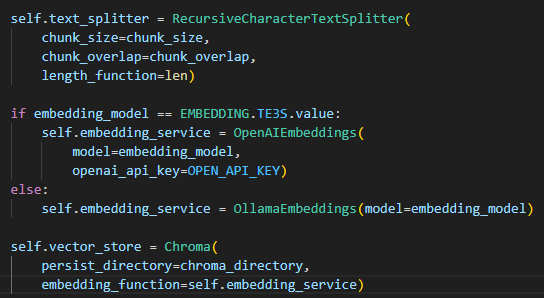
\includegraphics[width=0.8\textwidth]{imagenes/0070_chatbot_const_3.png}
                \caption{Clase Chatbot. Configuración de varios parámetros: text\_splitter, modelo de embedding y modelo de recuperación}		
                \label{fig:0070_chatbot_const_3}
            \end{figure}

            \noindent La configuración de la estrategia de búsqueda no es tan simple, en la figura \ref{fig:0071_chatbot_const_4} podemos ver las opciones de configuración disponibles. Mientras que métodos como \textit{Similarity} o \textit{MMR} están incluidas por defecto por Chroma, necesitamos usar clases específicas para las demás.

            \noindent Las estrategias \textit{TF-IDF} y \textit{BM25} utilizan una metodología distinta, por lo que necesitan el uso de las clases \textit{TFIDFRetriver} \cite{0032_tfidf} y \textit{BM25Retriever} \cite{0033_bm25} para funcionar correctamente.

            \noindent La estrategia de recuperación en grafo usa la clase \textit{GrapRetriever} \cite{0034_graphrag}, en la que usamos algunos metadatos obtenidos de los documentos para filtrar y recuperar documentos con metadatos similares.

            \begin{figure}[H]
                \centering
                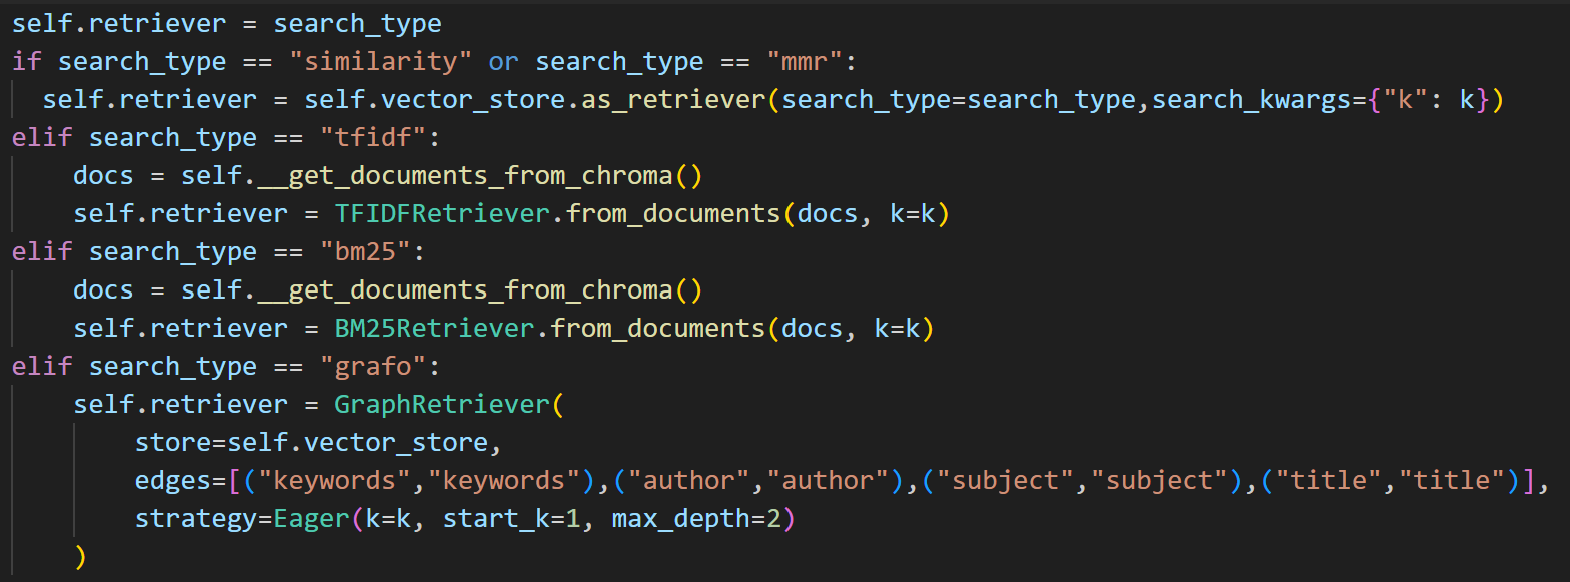
\includegraphics[width=1\textwidth]{imagenes/0071_chatbot_const_4.png}
                \caption{Clase Chatbot. Configuración de la estrategia de búsqueda}		
                \label{fig:0071_chatbot_const_4}
            \end{figure}

            \noindent La especificación del prompt es sencilla y se puede implementar en una sola línea (figura \ref{fig:0072_chatbot_const_5}. La clase \textit{PromptTemplate} ofrece multitud de métodos para este fin. El contenido de la variable \textit{prompt\_template} se puede ver al final de la sección \ref{sec:interfaz_chatbot} de esta memoria.

            \begin{figure}[H]
                \centering
                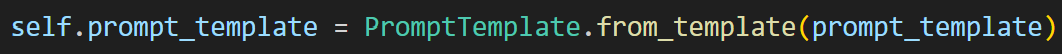
\includegraphics[width=0.8\textwidth]{imagenes/0072_chatbot_const_5.png}
                \caption{Clase Chatbot. Configuración del prompt}		
                \label{fig:0072_chatbot_const_5}
            \end{figure}

            \noindent La última de las configuraciones corresponde a la del modelo para hacer \textbf{reranking} (figura \ref{fig:0073_chatbot_const_6}). Para ello necesitamos usar varias clases, y como parámetros: el modelo de reranking y el número de documentos que filtrará (\textit{top\_n}). 

            \noindent La variable \textit{compressor\_retriever} guarda la configuración del modelo de reranking junto con el modelo de recuperación escogido para esta iteración del sistema RAG. De modo que al llamarla, se producirá un ``doble" filtrado de los documentos: primero se producirá la recuperación de documentos normal, y seguido, el filtrado de los mejores documentos recuperados por parte del modelo reranker.

            \begin{figure}[H]
                \centering
                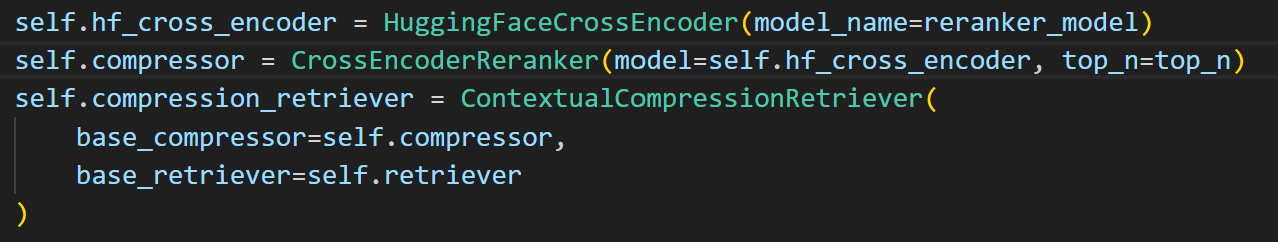
\includegraphics[width=0.9\textwidth]{imagenes/0073_chatbot_const_6.png}
                \caption{Clase Chatbot. Configuración del reranker}		
                \label{fig:0073_chatbot_const_6}
            \end{figure}

            \noindent Hemos podido ver en las figuras anteriores, la cantidad de integraciones que hemos usado para la configuración de los diferentes elementos de la clase \textit{Chatbot}. Como ya comentamos en la sección \ref{sec:LangChain}, esta es la gran ventaja que ofrece \textit{LangChain} respecto a otros frameworks, y que tenemos que aprovechar para facilitar el desarrollo de cualquier proyecto.

        \subsection{Interfaz de carga y actualización de la base de datos}

            En este apartado veremos como cargar y actualizar la base de datos vectorial del sistema RAG. Las siguientes imágenes, muestran fragmentos del código utilizado para su implementación. 

            \noindent En la siguiente figura podemos ver como se implementa parte de la interfaz usando \textit{Streamlit}. Hemos marcado tres bloques en la figura que pasaremos a explicar a continuación.

            \begin{figure}[H]
                \centering
                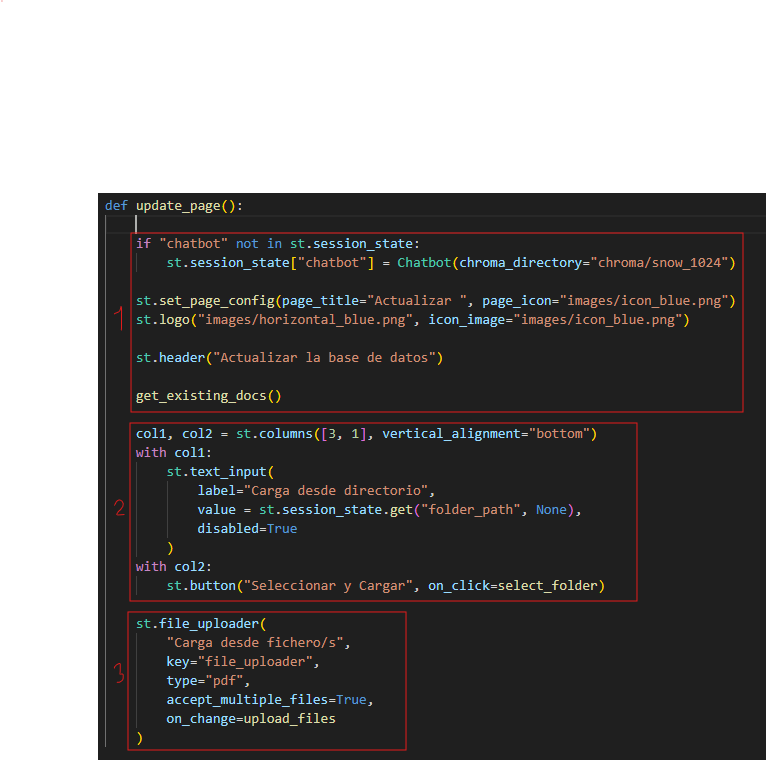
\includegraphics[width=1\textwidth]{imagenes/0074_update1.png}
                \caption{Interfaz. Código de la página de carga y actualización de la base de datos}		
                \label{fig:0074_update1}
            \end{figure}

            \noindent El primer bloque contiene la inicialización del \textit{Chatbot} junto con la configuración de logos y cabeceras de la página. \textit{Streamlit} provee de cantidad de recursos como se observa en el bloque, por ejemplo, cuenta con la variable \textit{session\_state} a la cual podemos asignar cualquier tipo variable sin temer perder los datos al actualizar la página.

            \noindent En los bloques dos y tres, añadimos a la interfaz estructuras que permiten subir documentos, ya sea desde directorio con la función \textit{select\_folder} (bloque dos) o simplemente cargando ficheros individuales y la función \textit{upload\_files} (bloque 3). Los ficheros usados para añadir documentos a la base de datos son automáticamente copiados a un directorio asignado en el constructor (\textit{docs\_directory}, figura \ref{fig:0069_chatbot_const_2}), creando así una base de referencias a las consultas de usuario.

            \noindent El resultado final de la interfaz se muestra en la siguiente figura. El código completo de esta página esta disponible en el repositorio \cite{0045_repo}, carpeta \textit{pages} en el archivo \textbf{update\_db.py}.

            \begin{figure}[H]
                \centering
                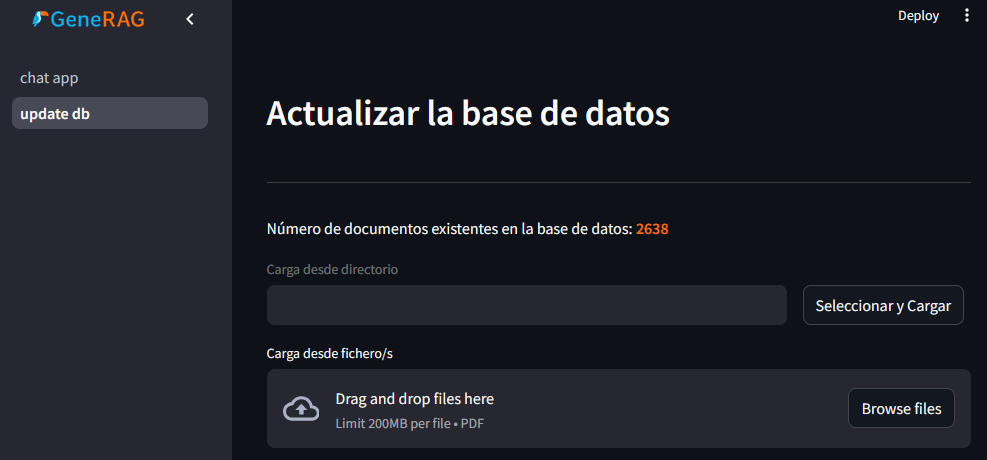
\includegraphics[width=.9\textwidth]{imagenes/0075_update2.png}
                \caption{Interfaz. Diseño de la página de carga y actualización de la base de datos}
                \label{fig:0075_update2}
            \end{figure}     

            \noindent En cuanto al código necesario para actualizar la base de datos, desarrollamos en la clase \textit{Chatbot} varias alternativas para incluir nuevos documentos. En la parte a) de la figura \ref{fig:0077_update_4} podemos ver la versión para cargar todos los documentos de un directorio, ya que usa la clase \textit{PyPDFDirectoryLoader} (la versión para cargar ficheros individuales es exactamente igual, salvo por la carga individual con \textit{PyPDFLoader}). También podemos observar como separa los documentos (\textit{text\_splitter}), genera diferentes IDs (\textit{\_\_calculate\_chunk\_ids}) y los incluye en la base de datos (\textit{vector\_store}).

            \noindent La parte b) de la misma figura muestra como se generan los IDs para los documentos, formándolos con partes de sus metadatos: nombre de archivo, número de página y número del fragmento en la página (depende del tamaño del chunk asignado, una página puede contener de 2 a 5 trozos). De esta forma obtenemos la referencia completa de donde ha obtenido la información el RAG ante una consulta de usuario (ver siguiente sección, figura \ref{fig:0096_interfaz5}).

            \begin{figure}[H]
                \centering
                \begin{subfigure}{0.49\textwidth}
                    \centering
                    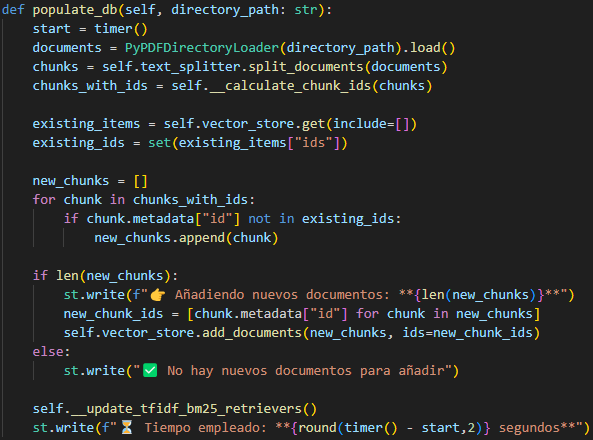
\includegraphics[width=1\textwidth]{imagenes/0076_update_3.png}
                    \caption{Método populate\_db}
                \end{subfigure}   
                \begin{subfigure}{0.49\textwidth}
                    \centering
                    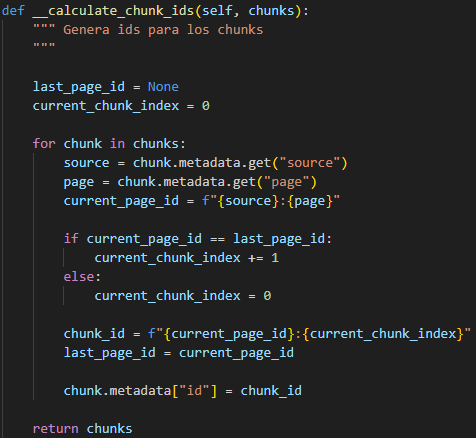
\includegraphics[width=1\textwidth]{imagenes/0077_update_4.png}
                    \caption{Método \_\_calculate\_chunk\_id}
                \end{subfigure}                  
                \caption{Clase Chatbot. Fragmentos de código de algunos de los métodos usados para actualizar la base de datos}
                \label{fig:0077_update_4}
            \end{figure}            

            \noindent El código de esta clase esta disponible en la carpeta \textit{classes} del repositorio \cite{0045_repo}, en el archivo \textbf{chatbot.py}. 

            \noindent Finalizaremos este apartado mostrando algunas figuras de los cuadros de diálogo diseñados al añadir archivos a nuestra base de datos.

            \begin{figure}[H]
                \centering
                
\includegraphics[width=.6\textwidth]{imagenes/0078_waiting.png}
                \caption{Interfaz. Cuadro de dialogo de tiempo de espera}		
                \label{fig:0078_waiting}
            \end{figure}

            \begin{figure}[H]
                \centering
                \begin{subfigure}{0.49\textwidth}
                    \centering
                    
\includegraphics[width=1\textwidth]{imagenes/0079_nomic_512.png}
                    \caption{nomic-embed-text}
                \end{subfigure}   
                \begin{subfigure}{0.49\textwidth}
                    \centering
                    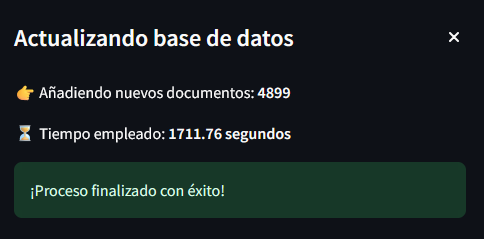
\includegraphics[width=1\textwidth]{imagenes/0079_bge_512.png}
                    \caption{bge-m3}
                \end{subfigure}    
                \begin{subfigure}{0.49\textwidth}
                    \centering
                    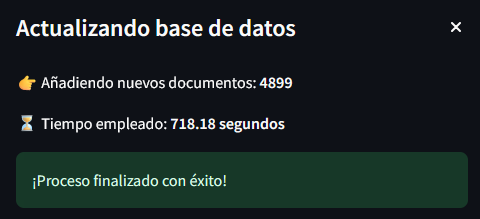
\includegraphics[width=1\textwidth]{imagenes/0079_jina_512.png}
                    \caption{jina-embeddings-v2-base-es}
                \end{subfigure}   
                \begin{subfigure}{0.49\textwidth}
                    \centering
                    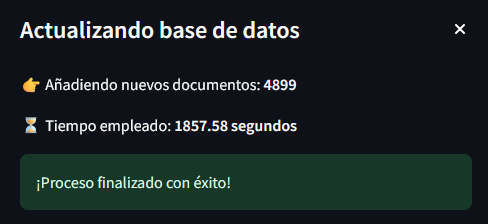
\includegraphics[width=1\textwidth]{imagenes/0079_snow_512.png}
                    \caption{snowflake-arctic-embed2}
                \end{subfigure}               
                \caption{Interfaz. Cuadros de dialogo. Tiempos para bases de datos con documentos de tamaño 512}
                \label{fig:0079_success1}
            \end{figure} 

            \begin{figure}[H]
                \centering
                \begin{subfigure}{0.49\textwidth}
                    \centering
                    
\includegraphics[width=1\textwidth]{imagenes/0079_nomic_1024.png}
                    \caption{nomic-embed-text}
                \end{subfigure}   
                \begin{subfigure}{0.49\textwidth}
                    \centering
                    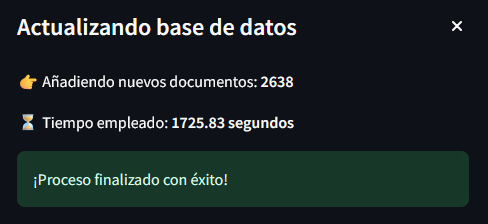
\includegraphics[width=1\textwidth]{imagenes/0079_bge_1024.png}
                    \caption{bge-m3}
                \end{subfigure}    
                \begin{subfigure}{0.49\textwidth}
                    \centering
                    
\includegraphics[width=1\textwidth]{imagenes/0079_jina_1024.png}
                    \caption{jina-embeddings-v2-base-es}
                \end{subfigure}   
                \begin{subfigure}{0.49\textwidth}
                    \centering
                    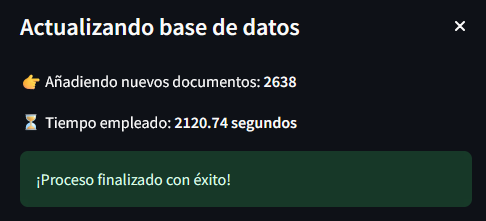
\includegraphics[width=1\textwidth]{imagenes/0079_snow_1024.png}
                    \caption{snowflake-arctic-embed2}
                \end{subfigure}               
                \caption{Interfaz. Cuadros de díalogo. Tiempos para bases de datos con documentos de tamaño 1024}
                \label{fig:0079_success2}
            \end{figure} 

            \noindent Si nos fijamos en las figuras \ref{fig:0079_success1} y \ref{fig:0079_success2}, destaca la diferencia de tiempo existente entre el par nomic-jina y bge-snowflake, siendo estos últimos los que más tiempo consumen al incluir nuevos documentos en la base de datos vectorial. El motivo para esta diferencia puede residir en una metodología más compleja para vectorizar los documentos de este último par, puesto que son los modelos más pesados en comparación.
            
            \noindent En contraste con los modelos locales, el tiempo de embedding del modelo \textit{text-embedding-3-small} (OpenAI) es extremadamente rápido. Como se puede observar en la figura \ref{fig:0099_te3s-embed}, el modelo vectoriza todos los documentos en solo 40 segundos.
            
            \begin{figure}[H]
            	\centering
            	
\includegraphics[width=.6\textwidth]{imagenes/0099_te3s-embed.png}
            	\caption{Interfaz. Tiempo de embedding de \textit{text-embedding-3-small}}		
            	\label{fig:0099_te3s-embed}
            \end{figure}

        \subsection{Interfaz del chatbot: Recuperación y generación de información}  
        \label{sec:interfaz_chatbot}

            En este apartado explicaremos el funcionamiento de la interfaz del chatbot del sistema RAG, mostrando los apartados correspondientes a la recuperación y generación de información especialmente. Ayudándonos de \textit{Streamlit}, se ha implementado página principal (figura \ref{fig:0080_interfaz_main}) con dos elementos personalizables: modelo de lenguaje y estrategia de búsqueda; y el chat.

            \begin{figure}[H]
                \centering
                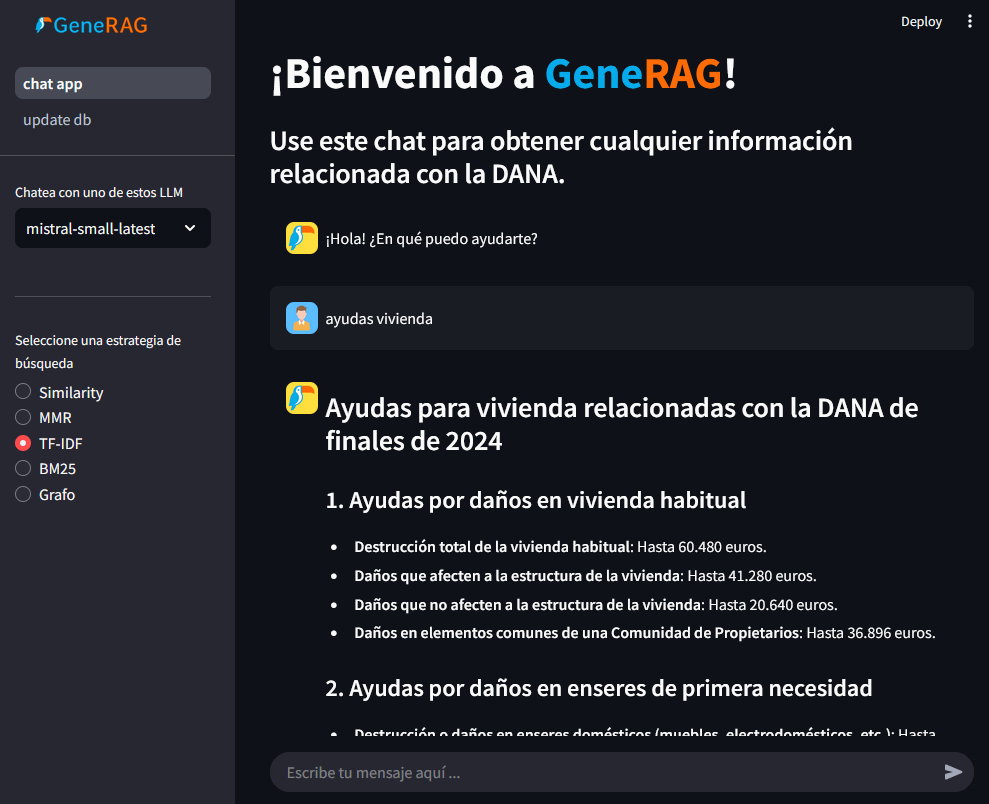
\includegraphics[width=1\textwidth]{imagenes/0080_interfaz_main.png}
                \caption{Interfaz. Página principal}		
                \label{fig:0080_interfaz_main}
            \end{figure}

            \noindent En la figura \ref{fig:0080_interfaz_main} se pueden observar los elementos los elementos mencionados en el párrafo anterior, situados en la barra lateral izquierda; ademas del chat con una conversación entre el usuario y el sistema RAG. A continuación, pasaremos a explicar el funcionamiento interno de estos elementos proporcionados por \textit{Streamlit} y también, las partes de recuperación y generación de información en la parte del chat.        

            \subsubsection{Configuración inicial del chatbot}

                \noindent Al igual que en la página de actualización de la base de datos (figura \ref{fig:0074_update1}), también necesitamos configurar el chatbot en la página principal.  
    
                \begin{figure}[H]
                    \centering
                    \begin{subfigure}{0.49\textwidth}
                        \centering
                        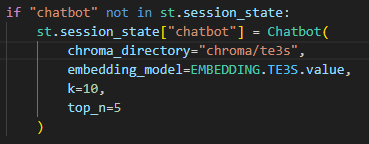
\includegraphics[width=1\textwidth]{imagenes/0081_chatbot.png}
                        \caption{Chatbot interfaz web}
                    \end{subfigure}   
                    \begin{subfigure}{0.49\textwidth}
                        \centering
                        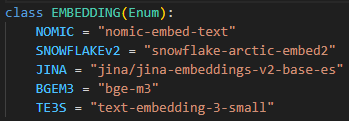
\includegraphics[width=1\textwidth]{imagenes/0081_embeddings.png}
                        \caption{Clase EMBEDDING}
                    \end{subfigure}                  
                    \caption{Fragmentos de código. Declaración de la variable Chatbot en la interfaz principal y clase EMBEDING}
                    \label{fig:0081_chatbot}
                \end{figure}   

                \noindent En la parte a de la figura anterior, se observan los detalles aportados para dicha configuración. Indicamos el modelo de embedding (del cual podemos elegir entre las opciones disponibles vistas en la parte b), los documentos recuperados (\textbf{k}) y los documentos filtrados por el reranker (\textbf{top\_n)}. Como se observa en la figura, este ejemplo usa el modelo de embedding \textit{text-embedding-3-small} junto un modelo de reranking, que se encargará de filtrar los cinco mejores documentos de los diez recuperados por el modelo de recuperación.

                \noindent La clase EMBEDDING esta situada en la carpeta \textit{classes}, en el fichero \textbf{LLM.py}. Los modelos de embedding disponibles deben ser descargados con antelación mediante Ollama (sección \ref{sec:ollama}) a excepción del modelo \textit{text-embedding-3-small}, del cual necesitaremos aportar nuestra clave de OpenAI.

            \subsubsection{Elementos de selección: selectbox y radio}  

                \textit{Streamlit} ofrece en su documentación oficial multitud de componentes que podemos usar en la interfaz web. Como se observó en la figura \ref{fig:0080_interfaz_main}, hemos usado una caja de selección (\textit{selectbox}) para elegir el modelo de lenguaje con el que chatear, y botones de radio (\textit{radio}) para escoger la estrategia de búsqueda del modelo de recuperación.

                \noindent El código mostrado en la parte a de la figura \ref{fig:0082_llms}, muestra la implementación de la caja de selección. La etiqueta \textit{sidebar} indica a Streamlit, que debe estar situado en la barra lateral, normalmente situada a la izquierda.

                \noindent De entre los parámetros, destacan: 

                \begin{itemize}
                    \item \textbf{options:} Lista de elementos que muestra la caja de selección (parte b, figura \ref{fig:0082_llms}).
                    \item \textbf{key:} Variable de \textit{session\_state} que tomará el valor determinado en la caja de selección.
                    \item \textbf{on\_change:} Función que se activará cuando cambie el valor de la caja de selección.
                \end{itemize}
    
                \begin{figure}[H]
                    \centering
                    \begin{subfigure}{0.49\textwidth}
                        \centering
                        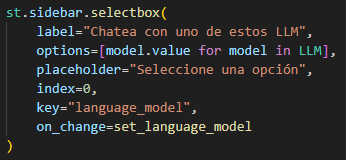
\includegraphics[width=1\textwidth]{imagenes/0082_selectbox.png}
                        \caption{Selectbox LLMs}
                    \end{subfigure}   
                    \begin{subfigure}{0.49\textwidth}
                        \centering
                        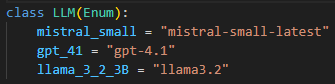
\includegraphics[width=1\textwidth]{imagenes/0082_llms.png}
                        \caption{Clase LLM}
                    \end{subfigure}                  
                    \caption{Fragmentos de código. Caja de selección de los modelos de lenguaje y clase LLM.}
                    \label{fig:0082_llms}
                \end{figure}        

                \noindent Los modelos disponibles vistos en la parte b de la figura \ref{fig:0082_llms}, han de ser descargados usando \textit{Ollama}; exceptuando los modelos de \textit{Mistral AI} y de \textit{OpenAI}, del cual necesitamos un código de su API.

                \noindent La función \textit{set\_language\_model} (figura \ref{fig:083_set_llm}) usa un método disponible en la clase Chatbot que cambia el modelo de lenguaje a usar por el RAG (figura \ref{fig:084_set_llm2}). Dicho método actua diferente según el modelo elegido, necesitando la clave API para los modelos de \textit{Mistral AI} y \textit{OpenAI}. El método es similar al aportado en el constructor, figura \ref{fig:0069_chatbot_const_2}.
    
                \begin{figure}[H]
                    \centering
                    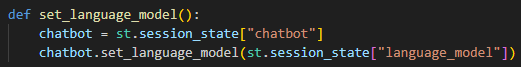
\includegraphics[width=.8\textwidth]{imagenes/083_set_llm.png}
                    \caption{Función de la interfaz. Modificar el modelo de lenguaje}		
                    \label{fig:083_set_llm}
                \end{figure}
    
                \begin{figure}[H]
                    \centering
                    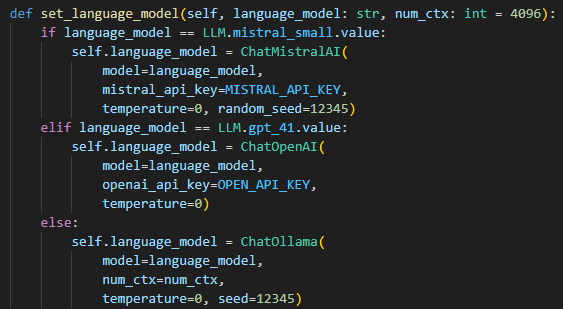
\includegraphics[width=.8\textwidth]{imagenes/084_set_llm2.png}
                    \caption{Clase Chatbot. Modificar el modelo de lenguaje}		
                    \label{fig:084_set_llm2}
                \end{figure}   

                \noindent La selección en radio, se implementa de forma similar (parte a de la figura \ref{fig:0084_radio}). Los valores entre los que seleccionar, en este caso han de ser aportados entre corchetes. Entre los demás parámetros destacan:

                \begin{itemize}
                    \item \textbf{key:} Variable de \textit{session\_state} que tomará el valor determinado en la selección de radio.
                    \item \textbf{on\_change:} Función que se activa al cambiar el valor de la selección de radio.
                \end{itemize}

                \noindent La función de la interfaz vista en la parte b de la figura \ref{fig:0084_radio}, activa el método de clase Chatbot para cambiar la estrategia de búsqueda. 
    
                \begin{figure}[H]
                    \centering
                    \begin{subfigure}{0.49\textwidth}
                        \centering
                        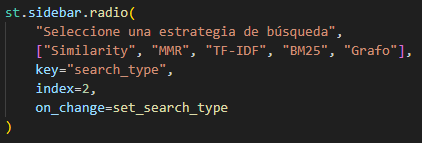
\includegraphics[width=1\textwidth]{imagenes/0084_radio_1.png}
                        \caption{Selección de radio, estrategias de búsqueda}
                    \end{subfigure}   
                    \begin{subfigure}{0.49\textwidth}
                        \centering
                        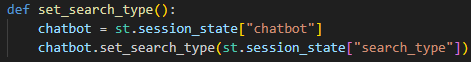
\includegraphics[width=1\textwidth]{imagenes/0084_radio_2.png}
                        \caption{Función de la interfaz}
                    \end{subfigure}                  
                    \caption{Fragmentos de código. Selección de radio para las estrategias de búsqueda y función de la interfaz para cambiarlas}
                    \label{fig:0084_radio}
                \end{figure}        
    
                \noindent Como se observa en la figura siguiente, cada estrategia cambia el método de recuperación (\textit{retriever}). Las estrategias \textit{similarity} y \textit{mmr} son traidas por defecto en la base de datos Chroma, mientras que para las demás tenemos que usar clases externas: \textit{TFIDFRetriever}, \textit{BM25Retriever} y \textit{GraphRetriever}. (El método es similar al aportado en el constructor, figura \ref{fig:0071_chatbot_const_4}).
    
                \begin{figure}[H]
                    \centering
                    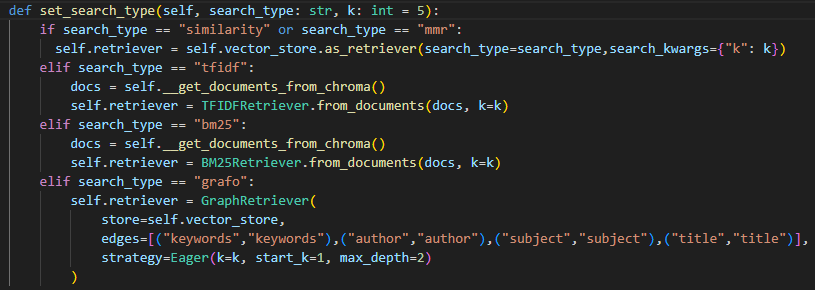
\includegraphics[width=.9\textwidth]{imagenes/0085_radio_3.png}
                    \caption{Clase Chatbot. Modificar la estrategia de búsqueda}		
                    \label{fig:0085_radio_3}
                \end{figure}            

            \subsubsection{Recuperación y generación de información}

                La parte dedicada a la interfaz del chatbot consta de varios bloques diferenciados, como se puede observar en la figura \ref{fig:0086_chat_codigo}. 
                
                \noindent En las primeras dos líneas (85-86) se crea la variable \textit{chat\_history} si no se encuentra disponible en la variable de sesión \textit{session\_state}, y le agrega un mensaje del sistema dando la bienvenida al chat. En dicha variable iremos guardando todo el historial de conversación entre el usuario y el sistema.

                \noindent El bucle for de las líneas 88 a 94 recorre cada mensaje disponible en la variable de sesión \textit{chat\_history}. Cada mensaje es diferenciado entre sistema y usuario (\textit{AIMessage} y \textit{HumanMessage}), y son impresos con distintos avatares según corresponda.

                \noindent La variable \textit{user\_query} de la línea 96, guarda la consulta hecha por el usuario. Esta consulta es retornada gracias al elemento de \textit{Streamlit} \textit{chat\_input}, que genera una entrada de texto flotante en la interfaz y en la que se puede escribir.

                \noindent A continuación, dicha entrada de texto se agrega al historial de conversación marcada como mensaje de usuario (\textit{HumanMessage}). Genera la respuesta del sistema llamando a la función \textit{query} (que explicaremos seguidamente), y agrega la respuesta al historial de conversación como \textit{AIMessage}. 
    
                \begin{figure}[H]
                    \centering
                    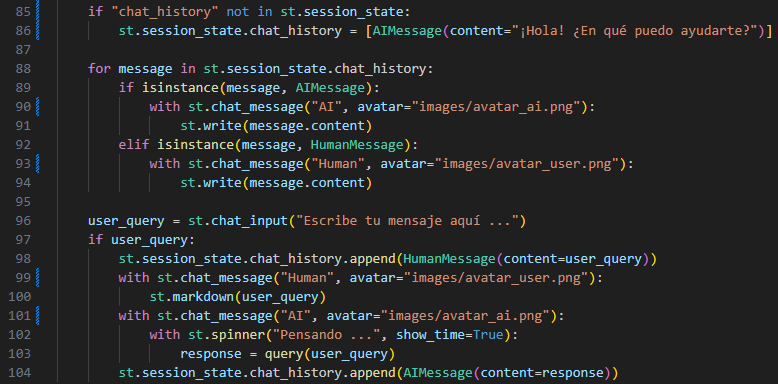
\includegraphics[width=.9\textwidth]{imagenes/0086_chat_codigo.png}
                    \caption{Fragmento de código correspondiente a la interfaz del chatbot}		
                    \label{fig:0086_chat_codigo}
                \end{figure}

                \noindent En la función \textit{query} vista en la figura \ref{fig:0087_chat_query}, suceden ambos procesos de recuperación y generación de información. La recuperación se da entre las líneas 20 a la 23, y la generación en la 42; pero entre ellas se producen otros procesos que dan más detalle y riqueza a la respuesta, y que pasaremos a explicar con detenimiento.

                \noindent En las líneas 20 y 21 se consigue el modelo de recuperación (\textit{retriever}) usado por el \textit{chatbot}. En el ejemplo se usa un modelo de recuperación con un reranker, el cuál efectuará un doble filtrado de los documentos recuperados por el modelo principal. 
                
                \noindent El método para iniciar la recuperación se ve en la línea 23. Mediante \textit{invoke}, el \textit{retriever} seleccionará los documentos más relevantes a la consulta proporcionada por el usuario a través del parámetro \textit{question}.

                \noindent A continuación, guardamos el contexto recuperado por el modelo (línea 84), es decir, el contenido del texto de los documentos recuperados. También guardamos ciertos metadatos (línea 25-39) de los documentos. En el ejemplo, usamos el ID del documento para mostrarlo junto con la respuesta del sistema, ofreciendo así un extra de información y referencias al usuario de donde ha sido obtenida la información.

                \noindent Para finalizar con la figura \ref{fig:0087_chat_query}, queda explicar la generación de información. Se encuentra en la línea 42, realizandose mediante la llamada al método de la clase \textit{Chatbot} \textit{answer\_query} y aportando sólo dos parámetros: la pregunta (\textit{question}) y el contexto (\textit{context}). La respuesta se guarda en la variable \textit{response\_text} mediante la función \textit{write\_stream} provista por Streamlit, que genera una escritura en tiempo real (\textit{token} a \textit{token}).

                \noindent Las variables \textit{response\_text} y \textit{sources} son retornadas por esta función, que terminarán siendo agregadas al historial de conversación.
    
                \begin{figure}[H]
                    \centering
                    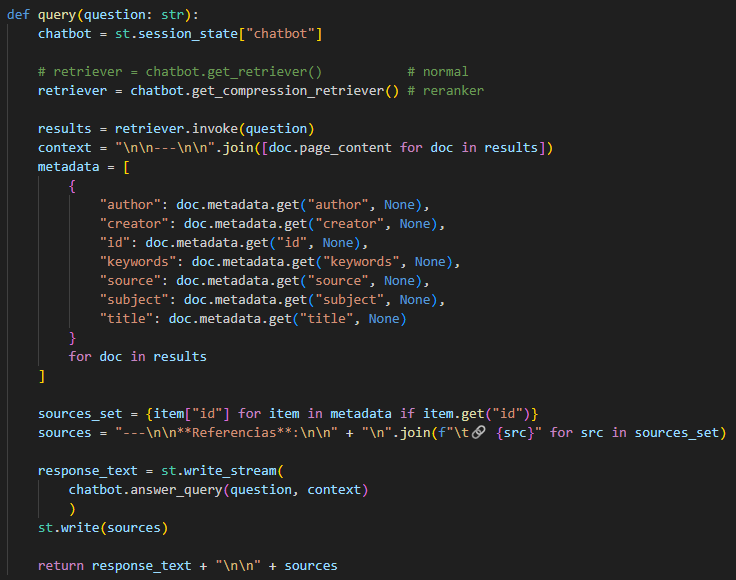
\includegraphics[width=.9\textwidth]{imagenes/0087_chat_query.png}
                    \caption{Función \textit{query} de la interfaz del chatbot. Hace los procesos de recuperación y generación de información del sistema RAG}		
                    \label{fig:0087_chat_query}
                \end{figure}

                \noindent La figura \ref{fig:0088_chat_answer} muestra el funcionamiento del método \textit{answer\_query} de la clase \textit{Chatbot}. En la figura podemos observar el funcionamiento de la cadena (\textit{query\_chain}) que nos brinda \textit{LangChain} para trabajar con modelos de lenguaje. En esta cadena podemos combinar el modelo de recuperación, los parámetros necesarios para el \textit{prompt}, la propia plantilla del prompt y el modelo de lenguaje. Generando así, la respuesta de forma más simple y eficiente con el comando \textit{stream}, que al igual que antes, genera la respuesta en tiempo real (\textit{token} a \textit{token}).
    
                \begin{figure}[H]
                    \centering
                    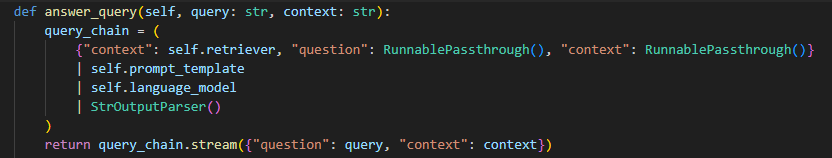
\includegraphics[width=.9\textwidth]{imagenes/0088_chat_answer.png}
                    \caption{Método \textit{answer\_query} de la clase Chatbot, retorna la respuesta del sistema RAG}		
                    \label{fig:0088_chat_answer}
                \end{figure}  

                \noindent Para finalizar este apartado, solo queda mostrar el \textit{prompt} usado por defecto por el \textit{chatbot}. La figura \ref{fig:0089_def_prompt} muestra la plantilla aplicada, en el ella se hace énfasis en el detalle y organización que deben presentar las respuestas. También se observan en las últimas dos líneas, como han de aportarse los argumentos con los que debe generar la respuesta: la pregunta y el contexto. 

                \noindent El planteamiento, instrucciones u órdenes escritas en el prompt, pueden generar distintas respuestas por el modelo de lenguaje. Por lo tanto, hay que buscar la forma adecuada para que el modelo de lenguaje obtenga mejores resultados.
    
                \begin{figure}[H]
                    \centering
                    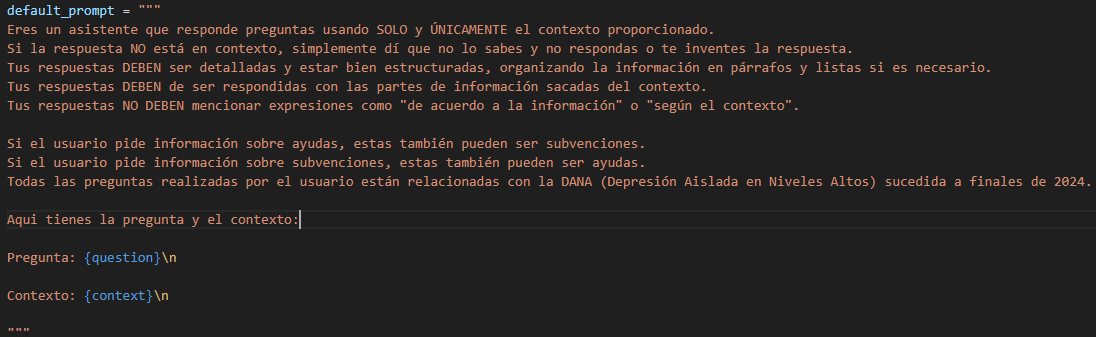
\includegraphics[width=1\textwidth]{imagenes/0089_def_prompt.png}
                    \caption{Prompt por defecto usado en el proyecto}		
                    \label{fig:0089_def_prompt}
                \end{figure}     

            \subsubsection{Capturas del chatbot}                   
    
                \begin{figure}[H]
                    \centering
                    
\includegraphics[width=.9\textwidth]{imagenes/0092_interfaz1.png}
                    \caption{Interfaz web del chatbot}		
                    \label{fig:0092_interfaz1}
                \end{figure}                   
    
                \begin{figure}[H]
                    \centering
                    
\includegraphics[width=.9\textwidth]{imagenes/0093_interfaz2.png}
                    \caption{Interfaz web con la barra lateral izquierda plegada}		
                    \label{fig:0093_interfaz2}
                \end{figure}                   
    
                \begin{figure}[H]
                    \centering
                    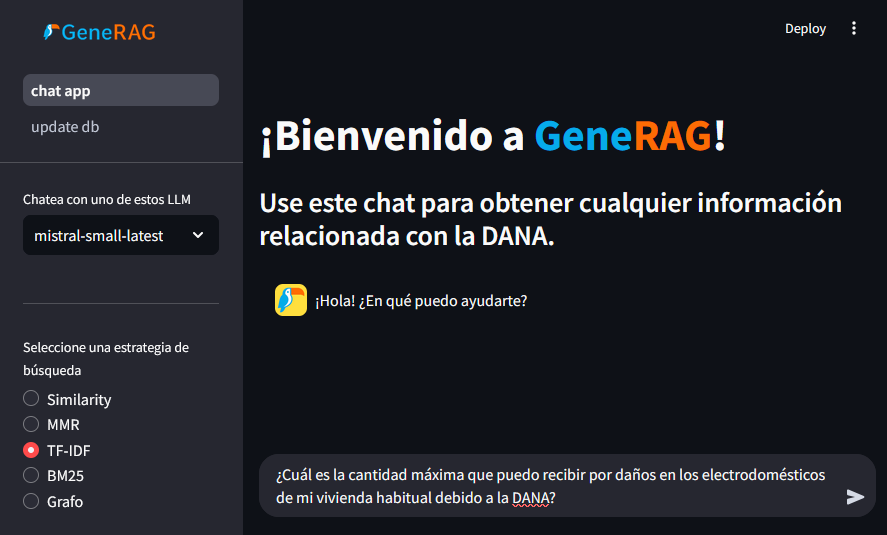
\includegraphics[width=.9\textwidth]{imagenes/0094_interfaz3.png}
                    \caption{Interfaz web con pregunta}		
                    \label{fig:0094_interfaz3}
                \end{figure}                   
    
                \begin{figure}[H]
                    \centering
                    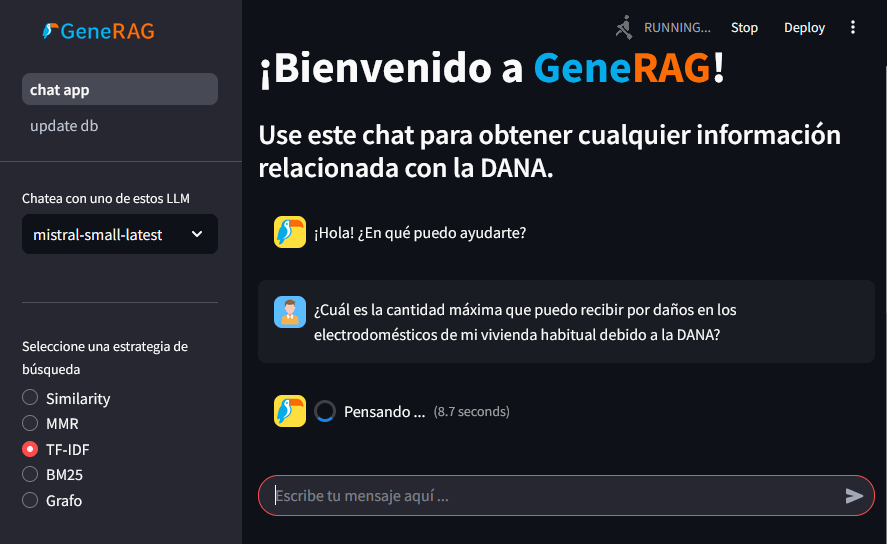
\includegraphics[width=.9\textwidth]{imagenes/0095_interfaz4.png}
                    \caption{Interfaz web generando respuesta}		
                    \label{fig:0095_interfaz4}
                \end{figure}                   
    
                \begin{figure}[H]
                    \centering
                    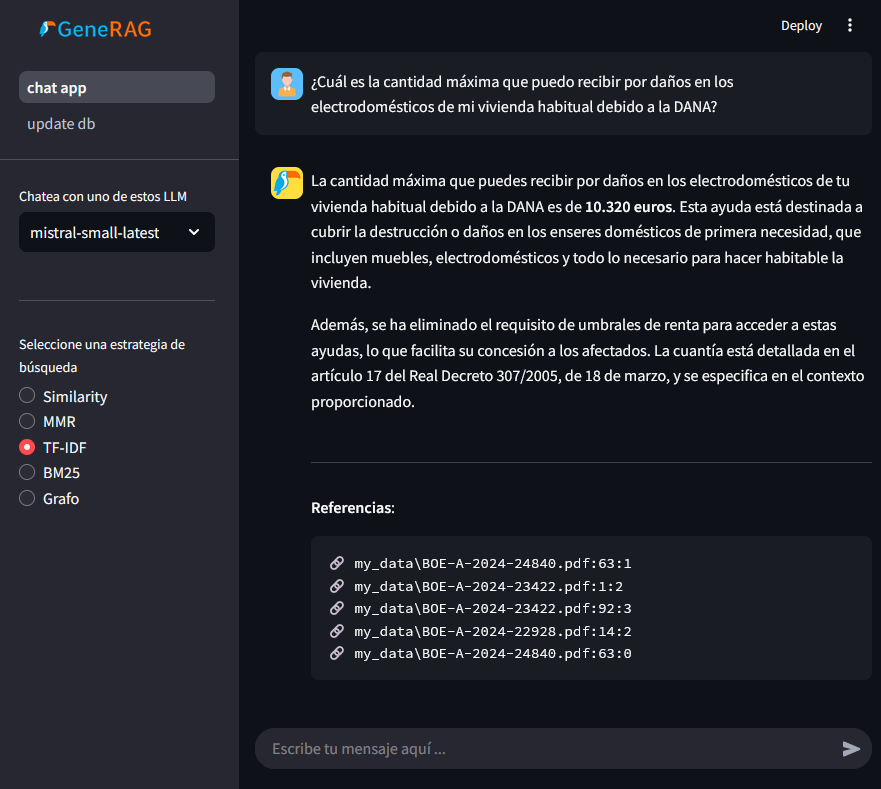
\includegraphics[width=.9\textwidth]{imagenes/0096_interfaz5.png}
                    \caption{Interfaz web con respuesta generada y referencias}		
                    \label{fig:0096_interfaz5}
                \end{figure}     
                
	\section{Conclusiones sobre el desarrollo de la aplicación}			
	
		El desarrollo de este proyecto ha puesto de manifiesto las claras ventajas de adoptar un enfoque basado en \textbf{RAG} frente a la solución planteada inicialmente: RASA. Como hemos comentado, RASA depende de un sistema de \textit{intents} y respuestas predefinidas, que exige un mantenimiento continuo y una anticipación de escenarios de interacción; el modelo con RAG ofrece una mayor versatilidad. Gracias a la integración continua con \textit{GitHub Actions}, la base de conocimiento se actualiza automáticamente con los documentos del BOE, lo que garantiza sincronización con la fuente original y reduce de forma significativa las tareas de mantenimiento.
		
		\noindent La incorporación de \textit{LangChain} resultó clave en la integración de los distintos componentes, facilitando las tareas de recuperación y generación de información. El proceso de desarrollo estuvo además favorecido por la abundante documentación y los numerosos tutoriales disponibles, lo que permitió una rápida implementación y conexión con diferentes plataformas de modelos de lenguaje.
		
		\noindent Por su parte, la interfaz desarrollada con \textit{Streamlit} ofreció una experiencia moderna y práctica. Su capacidad de generar aplicaciones web inyectando código \textit{Python} simplificó el trabajo, al permitir el uso de elementos interactivos habituales sin necesidad de programación adicional desde el \textit{backend}. De esta manera, se aceleró la construcción de la interfaz, la personalización y la adaptación del sistema a las necesidades específicas del proyecto.
		
		\noindent En conjunto, el nuevo enfoque proporciona un sistema más preciso, rápido y escalable. Así, se superan las limitaciones del marco anterior y se establece una solución sólida, eficiente y preparada para su evolución futura.

\endgroup
